\documentclass[%
	11pt,
	a4paper,
	utf8,
	%twocolumn
		]{article}	

\usepackage{style_packages/podvoyskiy_article_extended}


\begin{document}
\title{Пояснительная записка\\{\large Вычислительные техники решения задач линейного программирования в частично-целочисленной постановке и приемы работы с решателем SCIP}}

\author{\itshape Подвойский А.О., Глазунова Е.В.}


\date{}
\maketitle

\thispagestyle{fancy}

%Здесь приводятся заметки по специальным вопросам теории оптимизации

%\shorttableofcontents{Краткое содержание}{1}

\tableofcontents

\section{Ключевые термины и определения}

{Задача линейного программирования} (LP-задача) -- это ...

{Задача линейного программирования в частично-целочисленной постановке} (MILP-задача) -- это ...

\section{Ключевые компоненты платформы SCIP}

\subsection{Решатель SCIP. Общие сведения}

SCIP (Solving Constraint Integer Programs) \url{https://www.scipopt.org/} -- решатель, предназначенный для решения задач \emph{линейного} и \emph{нелинейного} программирования в частично-целочисленной постановке.

\subsubsection{Установка решателя SCIP}
Решатель проще всего установить вместе с оберткой PySCIPOpt \url{https://github.com/scipopt/PySCIPOpt} с помощью менеджеров \texttt{pip} или \texttt{conda}
\begin{lstlisting}[
	style = bash,
	numbers = none
	]
	$ pip install pyscipopt
	$ conda install -c conda-forge pyscipopt
\end{lstlisting}

\subsubsection{Приемы работы с решателем SCIP в интерактивной оболочке \texttt{scip}}

\subsubsection{Приемы работы с решателем SCIP через обертку PySCIPOpt}

Работа над задачей начинается с создания пустого экземпляра модели
\begin{lstlisting}[
style = ironpython,
numbers = none
]
import pyscipopt

model = pyscipopt.Model()
\end{lstlisting}

На созданном экземпляре можно вызывать методы чтения модели, конфигурационного файла параметров решателя и т.д.
\begin{lstlisting}[
style = ironpython,
numbers = none,
]
model.readProblem("./problem.lp")
model.readParams("./scip.set")
...
\end{lstlisting}



\subsection{Декомпозиционный решатель GCG. Общие сведения}

GCG \url{https://gcg.or.rwth-aachen.de/#about} -- это универсальный декомпозиционный решатель для задач линейного программирования в частично-целочисленной постановке, расширающий возможности базового решателя SCIP.

Он выявляет структуры в модели, к которым могут быть применены \emph{переформулировка Данцига-Вольфе} или \emph{декомпозиция Бендера}.

Модфицированная постановка задачи (после переформулировки Данцига-Вольфе) решается с помощью обобщения метода ветвей-и-границ, а именно с помощью метода ветвей-штрафов-секущих (branch-price-and-cut), включающего различные механизмы поиска решения -- превичные эвристики, стратегии ветвления, стратегии стабилизации, стратегии назначения штрафов и пр.

\subsubsection{Установка решетеля GCG}

Проще всего решатель установить вместе с обреткой PyGCGOpt \url{https://github.com/scipopt/PyGCGOpt} с помощью мендежера пакетов \texttt{conda}
\begin{lstlisting}[
style = bash,
numbers = none
]
$ conda install -c conda-forge pygcgopt
\end{lstlisting}



\subsubsection{Приемы работы с решателем GCG в интерактивной оболочке \texttt{gcg}}

Прочитать постановку задачи
\begin{lstlisting}[
style = bash,
numbers = none
]
GCG> read problem.lp
\end{lstlisting}

Запустить процедуру редуцированния размерности
\begin{lstlisting}[
style = bash,
numbers = none
]
GCG> presolve
\end{lstlisting}

Запустить процедуру поиска структур в матрице ограничений
\begin{lstlisting}[
style = bash,
numbers = none
]
GCG> detect
\end{lstlisting}

Записать постановку задачи сниженной размерности для \texttt{gnuplot}
\begin{lstlisting}[
style = bash,
numbers = none
]
GCG> write problem problem_reduced.gp
\end{lstlisting}

Фрагмент gp-файла
\begin{lstlisting}[
style = bash,
numbers = none
]
set encoding utf8
set terminal pdf
set output "problem_reduced.pdf"
set xrange [-1:506441]
set yrange[347788:-1]
set object 1 rect from 0,0 to 506441,183384 fc rgb "#1340C7"
set object 3 rect from 163304,183384 to 163306,183385 fc rgb "#718CDB" 
set object 4 rect from 163306,183385 to 163308,183386 fc rgb "#718CDB" 
set object 5 rect from 163308,183386 to 163310,183387 fc rgb "#718CDB" 
set object 6 rect from 163310,183387 to 163312,183388 fc rgb "#718CDB" 
set object 7 rect from 163312,183388 to 163314,183389 fc rgb "#718CDB" 
set object 8 rect from 163314,183389 to 163316,183390 fc rgb "#718CDB" 
set object 9 rect from 163316,183390 to 163318,183391 fc rgb "#718CDB" 
set object 10 rect from 163318,183391 to 163320,183392 fc rgb "#718CDB" 
set object 11 rect from 163320,183392 to 163322,183393 fc rgb "#718CDB" 
...
\end{lstlisting}

Создать pdf-файл декомпозиции задачи после шага снижения размерности
\begin{lstlisting}[
style = bash,
numbers = none
]
$ gnuplot problem_reduced.gp
\end{lstlisting}

\subsubsection{Приемы работы с решателем GCG через обертку PyGCGOpt}

\section{Выявленные баги SCIP и тонкости процедуры поиска решения}

\subsection{Недопустимое решение для релаксированной постановки задачи}

По состоянию на 18.06.2022 г. решатель SCIP версии 8.0.0 с оберткой PySCIPOpt версий 4.0.0 и 4.2.0 для операционной системы Windows 10 \emph{релаксированную постановку задачи} (т.е. при снятых ограничениях на целочисленность переменных) оценивает как неспособную привести к допустимому решению.

SCIP версии 7.0.3 (PySCIPOpt 3.4.0) как на операционной системе Windows 10, так и на Unix-подобных операционных системах (в частности, MacOS Monterey 12.1 и Linux Centos 7) решает задачу в релаксированной постановке корректно.

\subsection{Неединственность релаксированного решения}

Если эвристические приемы строятся на базе релаксированного решения задачи, важно помнить, что релаксированные решения, полученные с помощью различных решателей с точки зрения распределения значений переменных могут существенно различаться\footnote{Потому как гиперплоскость целевой функции может касаться политопа не в вершине, а по грани}, не смотря на то, что во всех случах зазор будет нулевым и целевая функция будет имееть одно и тоже значение (с оговоркой на допуск точности решателя). 

\subsection{Замечание о стабильности работы решателя SCIP на различных операционных системах}

\begin{itemize}
	\item Вычислительные эксперименты проводились на трех версиях решателя SCIP (7.0.0, 7.0.3, 8.0.0) и трех платформах: Windows~10, MacOS (Monterey~12), Linux (Centos~7). Разброс времени поиска решения для каждой конфигурации решателя оценивается минимум по 3 запускам сценария
	
	\item На текущий момент наиболее стабильные и наиболее адекватные результаты получаются
	\begin{itemize}
		\item для ОС Linux (Centos 7) и ОС MacOS (Monterey12) на решателе SCIP версии 7.0.3 (обертка PySCIPOpt 3.4.0) и платформе Ecole версии 0.7.3 , собранных для однопоточной реализации
		
		\item для ОС Windows 10 на решателе SCIP версии 8.0.0 (обертка PySCIPOpt 4.0.0), собранном для однопоточной реализации
	\end{itemize}
	
	\item Последняя доступная версия решателя SCIP 8.0.0 (PySCIPOpt 4.1.0) на MacOS (Monterey 12.1) и Linux (Centos 7) при тех же настройках, что и для SCIP версии 7.0.3, как правило, работает значительно медленнее (2.5-2.85 раза) и в большинстве случаев либо не успевает найти решение за отведенное время, либо «просаживает» целевую функцию
\end{itemize}



\section{Приемы поиска решения}

\subsection{Прием фиксации бинарно-целочисленных переменных в релаксированном решении}\label{sec:bin_int_relax_fix}

Часто фиксация целочисленных переменных\footnote{Вообще говоря, фиксировать можно не только бинарные и целочисленные переменные} в релаксированном решении приводит к приемлемому допустимому целочисленному решению, которое потом можно использовать как <<теплый старат>> или как базовое решение для других схем фиксации.
\begin{lstlisting}[
style = ironpython,
numbers = none
]
ZERO = 0.0
...
relax_sol: pd.Series = read_relax_sol(path_to_relax_sol)

model = pyscipopt.Model()
model.readProblem(path_to_lp_file)
model.readParams(path_to_set_file)

all_vars: t.List[pyscipopt.scip.Variable] = model.getVars()
bin_vars: t.List[pyscipopt.scip.Variable] = extract_vars_set_type(all_vars, BINARY)
int_vars: t.List[pyscipopt.scip.Variable] = extract_vars_set_type(all_vars, INTEGER)

all_zero_bin_vars: t.List[
	pyscipopt.scip.Variable
] = extract_from_relax_sol_zero_vars(
	relax_sol,
	sub_group_vars=bin_vars,
)
all_zero_int_vars: t.List[
	pyscipopt.scip.Variable
] = extract_from_relax_sol_zero_vars(
	relax_sol,
	sub_group_vars=int_vars,
)

for var in all_zero_bin_vars + all_zero_int_vars:
	model.fixVar(var, ZERO)

model.optimize()
...
\end{lstlisting}


\subsection{Прием подавления подгруппы первичных эвристик низкой эффективности}\label{sec:suh}

В некоторых случаях отдельные первичные эвристики могут оказаться не способными справится со своей задачей, не оказывая никакого влияния на процедуру поиска решения, и все же потреблять предоставленные ресурсы.

Такие эвристики -- условимся их называть первичными эвристиками низкой эффективности (ПЭНЭ) -- можно выявить путем анализа статистической сводки \verb|stat|-файла в разделе Primal Heuristics
\begin{lstlisting}[
title = {\sffamily Фрагмент файла статистической сводки 337\_bin\_default.stat},
style = bash,
numbers = none
]
...
Primal Heuristics  :   ExecTime  SetupTime      Calls      Found       Best
  LP solutions     :       0.00          -          -          0          0
	relax solutions  :       0.00          -          -          0          0
	pseudo solutions :       0.00          -          -          0          0
	...
	conflictdiving   :       0.00       0.00          0          0          0
	crossover        :       0.00       0.00          0          0          0
	dins             :       0.00       0.00          0          0          0
	distributiondivin:       0.00       0.00          0          0          0
	dualval          :       0.00       0.00          0          0          0
	farkasdiving     :    2032.89       0.00          1          0          0  # <- NB
	feaspump         :     882.12       0.00          1          0          0  # <- NB
	fixandinfer      :       0.00       0.00          0          0          0
	...
	intdiving        :       0.00       0.00          0          0          0
	intshifting      :      52.99       0.00          1          1          1
	...
\end{lstlisting}

В данном случае ПЭНЭ являются \texttt{farkasdiving} и \texttt{feaspump}. Чтобы подавить эти эвристики при следующем запуске \texttt{SCIP}, достаточно включить следующие строки в конфигурационный файл \texttt{scip.set}\footnote{При запуске интерактивной сесии через утилиту командной строки \texttt{scip}, решатель ищет этот файл в текущей директории и, если находит, автоматически вычитывает. При работе через PySCIPOpt требуется явно передавать путь до файла методу модели \texttt{readParams()}}
\begin{lstlisting}[
title = {\sffamily scip.set},
style = bash,
numbers = none
]
...
heuristics/farkasdiving/freq = -1
heuristics/feaspump/freq = -1
...
\end{lstlisting}

Доступ к статистической сводке можно получить либо в сессии \texttt{SCIP}, либо через одну из оберток над решателем (например, с помощью PySCIPOpt)
\begin{lstlisting}[
title = {\sffamily Фрагмент сессии scip. Получение статистической сводки},
style = bash,
numbers = none
]
...
SCIP> read file.lp
SCIP> opt
SCIP> display stat
\end{lstlisting}

\begin{lstlisting}[
title = {\sffamily Получение статистической сводки через обертку PySCIPOpt},
style = ironpython,
numbers = none
]
import pyscipopt

model = pyscipopt.Model()
model.readProblem("...")
model.readParams("...")
model.optimize()

model.printStatistics()
\end{lstlisting}





\subsection{Прием подбора порога бинаризации для бинарных переменных в релаксированном решении}\label{sec:find_bin_thresh}

Условимся \emph{фиксацией} называть стратегию инициализации подгруппы переменных $ x_k $ (вещественных, бинарных или целочисленных), значения которых задаются на основе каких-либо эврестических соображений, например, касающихся специальных свойств матрицы ограничений, и способных в результате привести к такой постановке задачи, которую, используя механизмы первичных эвристик, сепараторов, пропагаторов и пр. можно развить в \emph{допустимое целочисленное решение}.

Базовая идея построения \emph{фиксации на бинарных переменных} заключается в том, чтобы значения бинарных переменных в релаксированном решении\footnote{Верхний левый индекс <<$ r $>> указывает на релаксированное значение, а верхний правый <<$ (b) $>> -- на то, что речь идет о бинарной переменной} $ {\{{}^rx^{(b)}_k\}}_{k=1, \ldots} $ интерпретировать как \emph{степень уверенности} решателя в том, что рассматриваемую бинарную переменную можно выставить в единицу.

Если значение $ k $-ой бинарной переменной $ {}^rx_k^{(b)}$ превосходит некоторый \emph{порог}~$ \theta $, то переменная выставляется в единицу, в противном случае -- в ноль. Порог подбирается итерационно, начиная с некоторого нижнего значения $ \theta_l $ (по умолчанию $ \theta_l = 0 $), увеличивая текущее значение порога на величину шага $ \Delta \theta $ и заканчивая верхним значением порога $ \theta_u $ (по умолчанию $ \theta_u = 1 $).

Для практических целей достаточно остановится на наименьшем значении порога $ \theta $, который отвечает такой фиксации, которую решатель SCIP не отклоняет как неспособную привести к допустимому целочисленному решению.
\begin{lstlisting}[
title = {\sffamily Фрагмент лога решателя SCIP для случая фиксации, которую невозможно развить\\ в допустимое целочисленное решение},
style = bash,
numbers = none	
]
...
SCIP Status        : problem is solved [infeasible]
Solving Time (sec) : 3.00
Solving Nodes      : 0
Primal Bound       : +1.00000000000000e+20 (0 solutions)
Dual Bound         : +1.00000000000000e+20
Gap                : 0.00 %
original problem has 740251 variables (2666 bin, 147789 int, 0 impl, 589796 cont) and 545350 constraints
...
\end{lstlisting}

После того как порог $ \theta $ подобран, бинарные переменные разбиваются на две подгруппы: подгруппу бинарных переменных, выставленных в ноль $ \{x_k^{(b_0)}\} $, и подгруппу бинарных переменных, выставленных в единицу $ \{ x_k^{(b_1)} \} $. Долю бинарных переменных, выставленных в ноль обозначим через~$ \delta_{b_0} $, долю бинарных переменных, выставленных в единицу -- через $ \delta_{b_1} $, а целевую функцию, найденную при заданных долях -- через $ f_{\theta}(\delta_{b_0}, \delta_{b_1}) $.

В результате получаем исследовательский инструмент, который дает возможность управлять решением через подбор долей $ \delta_{b_0} $ и $ \delta_{b_1} $ при найденном пороге $ \theta $. Часто оказывается эффективным прием управления решением через подбор доли нулевых бинарных переменных $ \delta_{b_0} $.

Целевая функция, вычисленная при единичной доле нулевых бинарных переменных $ f_{\theta}(\delta_{b_0}=1) $, как правило, значительно уступает целевой функции релаксированного решения $ f_r $. Но тем неменее это решение может быть улучшено, сокращением доли $ \delta_{b_0} $ (см.~\pic{fig:a78cbeadfracbinzeros} и \pic{fig:337fracbinzeros}).

\begin{figure}[!h]
	\centering
	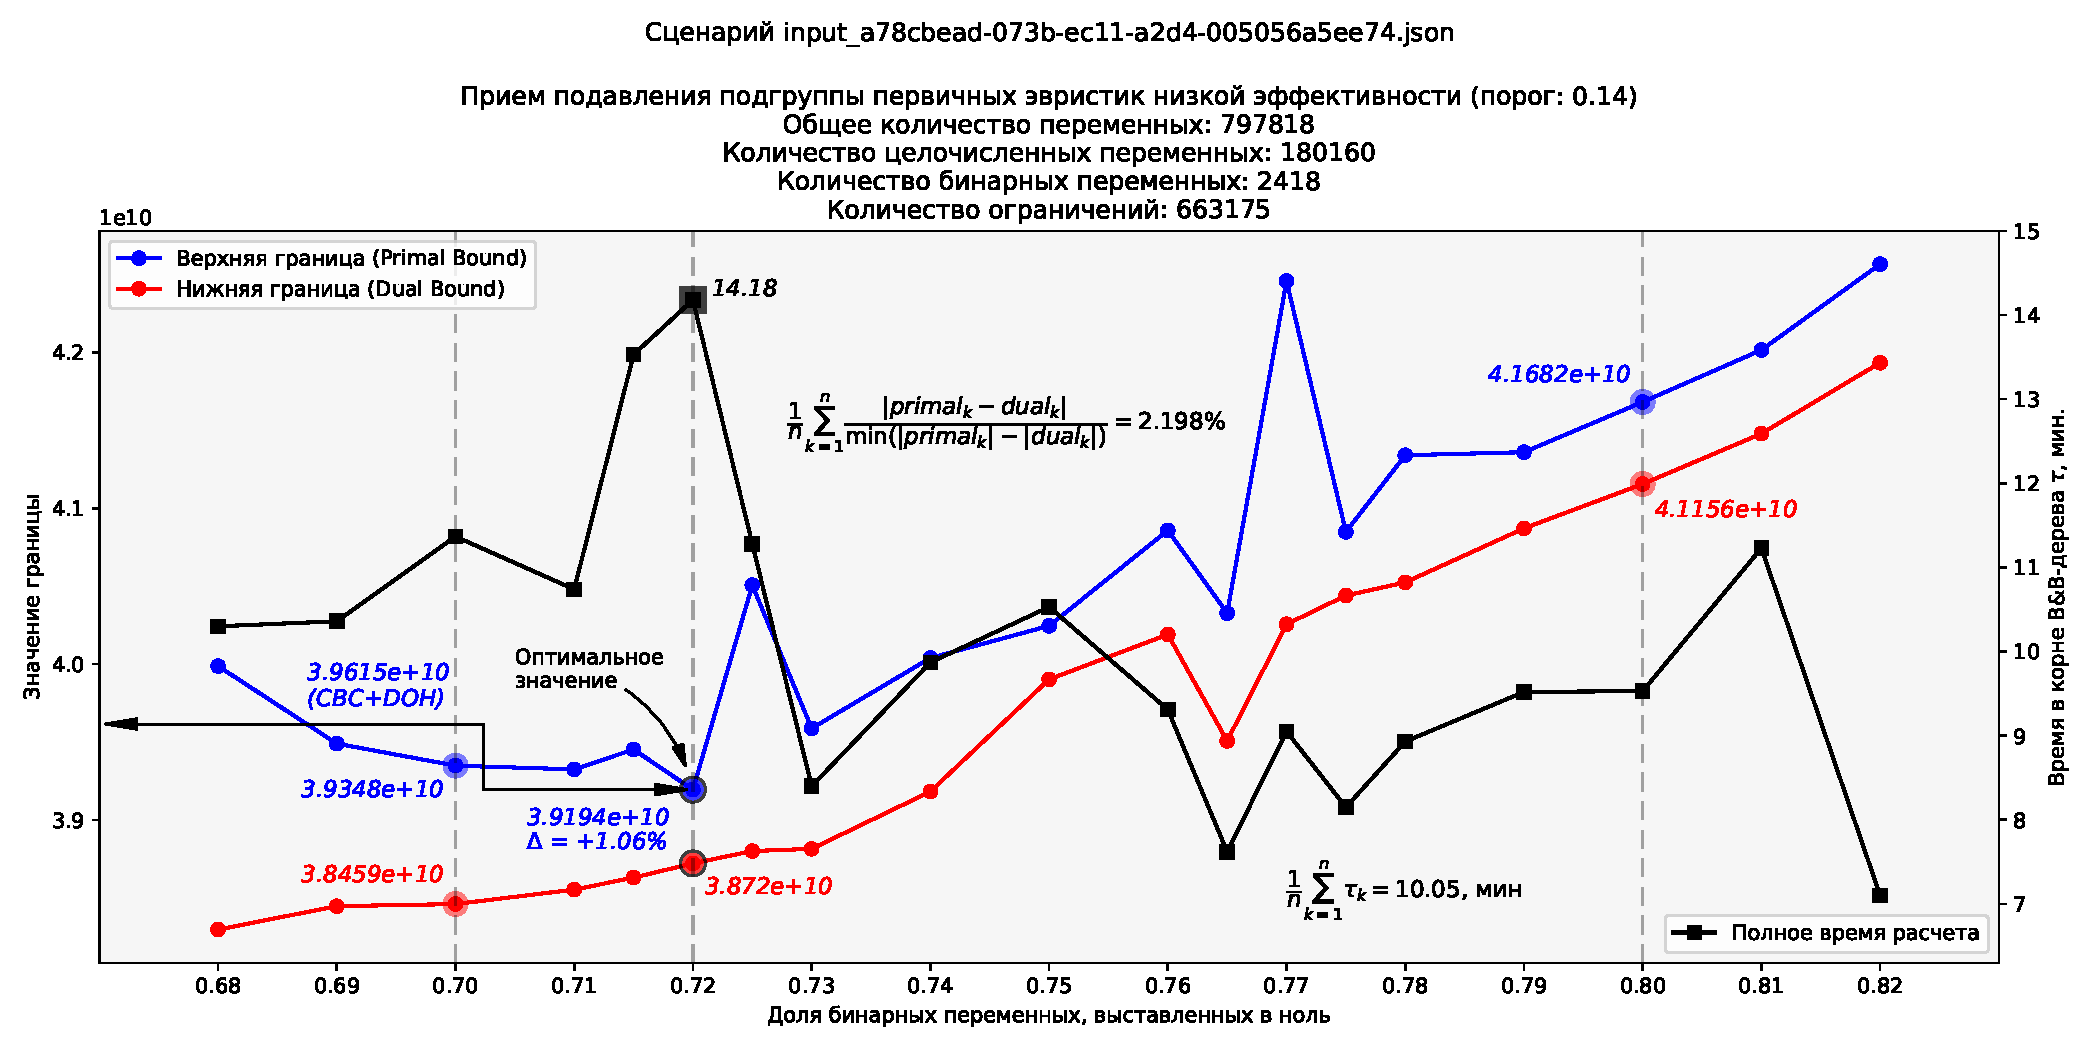
\includegraphics[scale=0.45]{figures/a78cbead_frac_bin_zeros.pdf}
	\caption{ Зависимость верхней границы решения от доли бинарных переменных, \\выставленных в ноль. Сценарий \texttt{a78cbead} }\label{fig:a78cbeadfracbinzeros}
\end{figure}

\begin{figure}[!h]
	\centering
	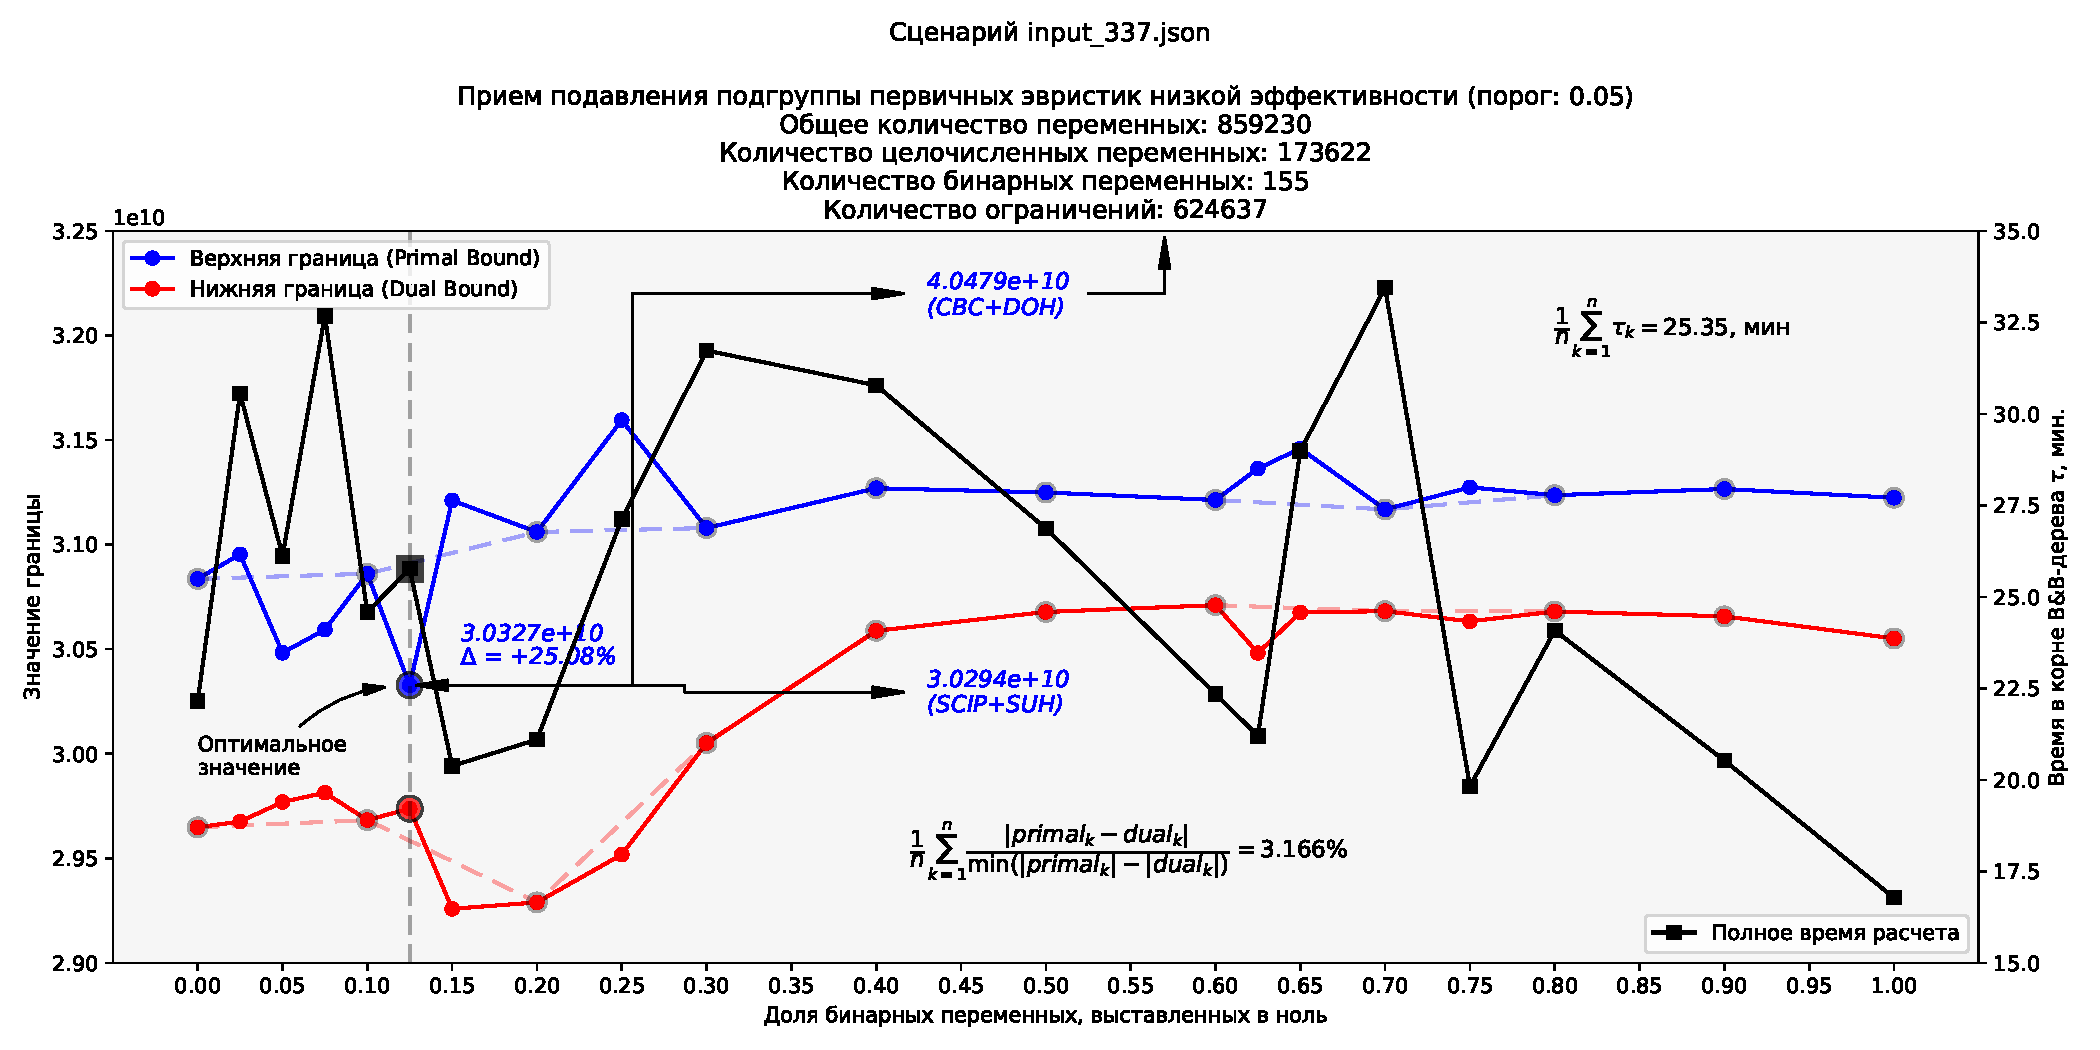
\includegraphics[scale=0.45]{figures/337_frac_bin_zeros.pdf}
	\caption{ Зависимость верхней границы решения от доли бинарных переменных, \\выставленных в ноль. Сценарий \texttt{337} }\label{fig:337fracbinzeros}
\end{figure}

Как видно из графиков, на кривой изменения верхней границы решения существует точка с наименьшим значением целевой функции $ f_{\theta}(\delta_{b_0}) $ допустимого целочисленного решения. Эта точка и будет <<оптимальной>> для рассматриваемого сценария.

\subsection{Методы машинного обучения в задачах комбинаторной оптимизации}

\subsubsection{Постановка задачи}

Цель: Разработать процедуру построения частично-заданного решения на фиксациях для сценариев с матрицей ограничений произольной структуры.

Вход: произвольная матрица ограничений\footnote{Предполагается, что матрица ограничений имеет низкую меру обусловленности}.

Выход: набор бинарных и целочисленных переменных, фиксация которых в ноль с высокой вероятностью приведет к допустимому целочисленному решению.

База: частично-заданное решение, построенное на фиксациях нулевых бинарных и целочисленных переменных в релаксированном решении.

\subsubsection{Стратегии решения задачи}

\paragraph{Стратегия №1} С помощью техник t-SNE и LLE найти низкоразмерное представление бинарно-целочисленных переменных. Оценить пермутационную важность признаков и важность признаков по Шепли.

Оценить меру похожести \emph{релаксированного решения} $ {}^r\{x_k\}_{k=1}^M $ и \emph{допустимого целочисленного решения} $ {}^f\{x_k\}_{k=1}^M $, например, с помощью \emph{коэффициента Отиаи}\footnote{\url{https://en.wikipedia.org/wiki/Cosine_similarity}}
\begin{align*}
	K = \bigg[ \dfrac{ \# {}^r\{x_k\}\bigcap {}^f\{x_k\} }{M} \bigg]^2, \quad K \in [0, 1],
\end{align*}
где $ {}^r\{x_k\} $ -- набор значений переменных в релаксированном решении; $ {}^f\{x_k\} $ -- набор значений переменных в допустимом решении; $ \# x \bigcap y $ -- количество переменных на пересечении решений $ x $ и $ y $; $ M $ -- количество переменных в сценарии.

Если релаксированное решение и допустимое целочисленное не пересекаются, то есть не имеют переменных с одним и тем же значением, то очевидно коэффициент Отиаи равен нулю. Если же решения пересекаются по всем переменным, то коэффициент становится равным единице. 

Задачу построения частично-заданного решения на фиксациях предлагается свести к задаче обнаружения аномалий в данных. Бинарные и целочисленные переменные, которые могут быть зафиксированны в ноль будем считать <<штатным>> режимом, а бинарные и целочисленные переменные, которые не могут -- аномалиями. Другими словами, задача сводится к отысканию бинарных и целочисленных переменных, которые не могут быть зафиксированы в ноль. Такие <<аномальные>> экзмепляры остаются без рекомендуемого значения для фиксации, а оставшиеся нулевые <<штатные>> бинарные и целочисленные переменные фиксируются в ноль и на этом процедура построения частично-заданного решения считается завершенной.

Для повышения надежности прогноза предлагается использовать ансамбль детекторов аномалий. Решение о фиксации бинарной или целочисленной переменной в ноль принимается на основании большинства голосов ансамбля детекторов.

Набор данных представляет собой неупорядоченную коллекцию матриц признакового описания, ассоциированных с соответствующими lp/mps-файлами математической постановки задачи (условимся называть их \emph{сценариями}).

Ансамбль детекторов аномалий обучается по роторной схеме:
\begin{itemize}
	\item На $ i $-ой итерации все матрицы признакового описания (всего в наборе $ S $ матриц/сценариев) кроме $ i $-ой матрицы используются для обучения детекторов, а на $ i $-ой матрице признакового описания строится прогноз аномальных экземпляров, которые помечаются как <<-1>>. В результате получается коллекция бинарных и целочисленных переменных, помеченных либо как <<0>>, либо как <<-1>>. Построенное решение сравнивается с допустимым целочисленным решением с помощью коэффициента Отиаи. Высокие значения коэффициента говорят о слабой согласованности. Если коэффициент Отиаи превосходит некоторый заданный порог, то полученная фиксация подается на вход решателю SCIP. Если фиксация не приводит к недопустимому решению, то выполняется попытка найти допустимое целочисленное решение за отведенное время. Если SCIP обнаруживает недопустимость схемы фиксации, то ключевые параметры детекторов обновляются в соответствии с определенной логикой и $ i $-ая итерация повторяется (можно ограничить число итераций-обновлений),
	
	\item Затем детекторы обучаются на следующем поднаборе $ S - 1 $ матриц признакового описания. На исключенной матрице снова строится прогноз аномальных экземпляров и т.д.
\end{itemize}

По окончании процедуры для каждого сценария будет создано частично-заданное решение на фиксациях, будет посчитан коэффициент Отиаи и либо будет найдено допустимое целочисленное решение, либо нет.

Полезно провести анализ влияния ключевых гиперпараметров детекторов на процедуру поиска решения.





\subsubsection{Концепт матрицы признакового описания бинарных и целочисленных переменных}

В качестве признаков бинарно-целочисленных переменных предлагается использовать:
\begin{enumerate}
	\item Значение переменной $ x_i $ в <<усредненном>> релаксированном решении\footnote{Задача линейного программирования в релаксированной постановке решается с использованием различных методов (двойственный симплекс-метод, метод внутренней точки и т.д.), а затем полученные решения усредняются},
	
	\item Модифицированную Z-оценку на <<усредненном>> релаксированном решении,
	
	\item Дробную часть значения переменной $ x_i $ в <<усредненном>> релаксированном решении,
	
	\item Пороги бинаризации на <<усредненном>> релаксированном решении (каждый порог это отдельный принак),
	
	\item Число ограничений $ n_i $, в которые входит рассматриваемая переменная $ x_i $,
	
	\item Число положительных $ n_i^{+} $ и отрицательных $ n_i^{-} $ коэффициентов в ограничениях, ассоциированных с рассматриваемой переменной $ x_i $,
	
	\item Булев маркер удаления переменной $ x_i $ после шага снижения размерности задачи,
	
	\item Коэффицент $ c_i $ при переменной $ x_i $ в целевой функции $ \mathbf{c}^T \mathbf{x} $,
	
	    \item Вероятность того, что $ i $-ая бинарная или целочисленная переменная $ x_i $ будет выставлена в~1 (индекс <<$ {-i} $>> означает без учета $ i $-ой переменной)
	\begin{align*}
		\mathbf{P}(x_i = 1) = \sigma \Bigg( \dfrac{1}{t} \, (\mathbf{c}^T \mathbf{x})_{-i} \Bigg),
	\end{align*}
где $ \sigma $ -- логистический сигмоид, $ t $ -- <<температура>> (чем выше температура, тем случайнее выход), $ \mathbf{c} $ -- вектор коэффициентов целевой функции, $ \mathbf{x} $ -- вектор переменных.

    \item Важность $ x_i $ переменной с точки зрения пресолверов.
\end{enumerate}



\section{Описание вычислительных экспериментов на сценариях группы ИКП}

На всех сценариях группы ИКП (как с бинарными переменными, так и без них) решения удавалось найти с помощью \emph{метаконфигурации} (см. раздел~\ref{sec:ikp_bins}), включающей прием подавления подгруппы первичных эвристик низкой эффективности и процедуру построения частично-заданного решения на фиксациях (для нулевых бинарных и целочисленных переменных). 

\subsection{Общие замечания по процедуре поиска решения на сценариях \emph{без} бинарных переменных}

Метаконфигурация\footnote{Под метаконфигурацией понимается совокупность конфигурации решателя и набора эвристических приемов} SUH (Suppress Useless Heuristics) процедуры поиска решения сводится к приему подавления подгруппы первичных эвристик низкой эффективности.

\remark{
Решение получено без доменно-ориентированных эвристик, <<теплого>> старта и подбора параметров решателя
}

Конфигурация решателя SCIP для всех сценариев группы ИКП (без бинарных переменных) имеет вид
\begin{lstlisting}[
	title = {\sffamily scip.set. Сценарии группы ИКП без бинарных переменных},
	style = bash,
	numbers = none,
	]
	# критерии останова и перезапуска
	limits/time = 7200
	limits/gap = 0.02  # решение останавливается при зазоре <= 2%
	
	# подавление подгруппы первичных эвристик низкой эффективности
	heuristics/farkasdiving/freq = -1
	heuristics/feaspump/freq = -1
	heuristics/randrounding/freq = -1
	heuristics/shiftandpropagate/freq = -1
	heuristics/shifting/freq = -1
\end{lstlisting}

Сводка результатов вычислительных экспериментов доступна по ссылке \url{https://docs.google.com/document/d/1V9fZLT9cXkbVQ5BvMCwzKrAiASZ2v4-01Z68jVBZUBU/edit?usp=sharing}.

\subsubsection{Сценарий \texttt{F398266B} без бинарных переменных}

\textbf{Статистика}\vspace*{1mm}

Общее количество переменных: 774901

Количество целочисленных переменных: 172449

Количество бинарных переменных: 0

Количество ограничений: 650263

lp-файл: \url{https://disk.yandex.ru/d/o_eAb9475u5ueg}

\vspace*{5mm}\textbf{Анализ решения}\vspace*{1mm}

Пул решений задачи был найден с помощью следующих первичных эвристик:
\begin{itemize}
	\item INTSHIFING,
	
	\item RENS.
\end{itemize}

Файл решения задачи (метаконфигурация SUH) доступен по ссылке \url{https://disk.yandex.ru/d/URRnZ8soTaJEgQ}

Файл статистической сводки (метаконфигурация SUH) доступен по ссылке \url{https://disk.yandex.ru/d/N2tfhj1N6RczzA}

Файл решения задачи (метаконфигурация FZBIVSUHPB) доступен по ссылке \url{https://disk.yandex.ru/d/-y7p5FyJyYirkw}

Файл статистической сводки (метаконфигурация FZBIVSUHPB) доступен по ссылке \url{https://disk.yandex.ru/d/1JaMC9aFjubDbA}

\vspace*{3mm}
\textbf{Вывод по сценарию}: описанная выше метаконфигурация SUH приводит к решению задачи, которое оказывается по отношению к результату на доменно-ориентированных эвристиках (\verb|USE_RECALCULATION_ON_FLOW=true|) для последнего решения из пула допустимых целочисленных решений (ОС Linux Centos 7) на 1.063\% лучше в смысле целевой функции и на 10.20\% -- в смысле временных издержек (\pic{fig:summary_f398266b}). 

Метаконфигурация FZBIVSUHPB (подробнее в разделе~\ref{sec:ikp_bins}) по отношению к тому же результату на доменно-ориентированных эвристиках дает решение задачи, которое на 1.155\% лучше в смысле целевой функции и на 65.27\% -- в смысле временных издержек (\tblref{tab:f398266b_wo_bins}).

Синим цветом обозначен выигрыш в процентах.

{
	%\rowcolors{2}{white}{lightgray!15}
	\begin{table}[!h]
		\centering
		\caption{Сводка результатов анализа эффективности \\метаконфигураций SUH и FZBIVSUHPB. Сценарий \texttt{f398266b} без бинарных переменных}
		\begin{tabular}{ p{2.5cm} p{3.3cm} p{3.4cm} }
			\emph{Способ} & \emph{Полное время расчета, мин} & \emph{Верхняя граница решения, $ \times 10^{10} $} \\
			\hline\hline\\[-3.5mm]
			{CBC+DOH} & 21.38 & $ 5.905048 $ \\
			\hline
			SCIP+SUH & 19.27 {\color{blue} $\ +9.87 $\%} & $ 5.842154 $ {\color{blue} $\ +1.065 $\%} \\
			\hline
			SCIP+FZB... & 9.43 {\color{blue} $\ +55.89 $\%} & $ 5.836815 $ {\color{blue} $\ +1.155 $\%} \\
		\end{tabular}\label{tab:f398266b_wo_bins}
	\end{table}
}

\begin{figure}[!h]
	\centering
	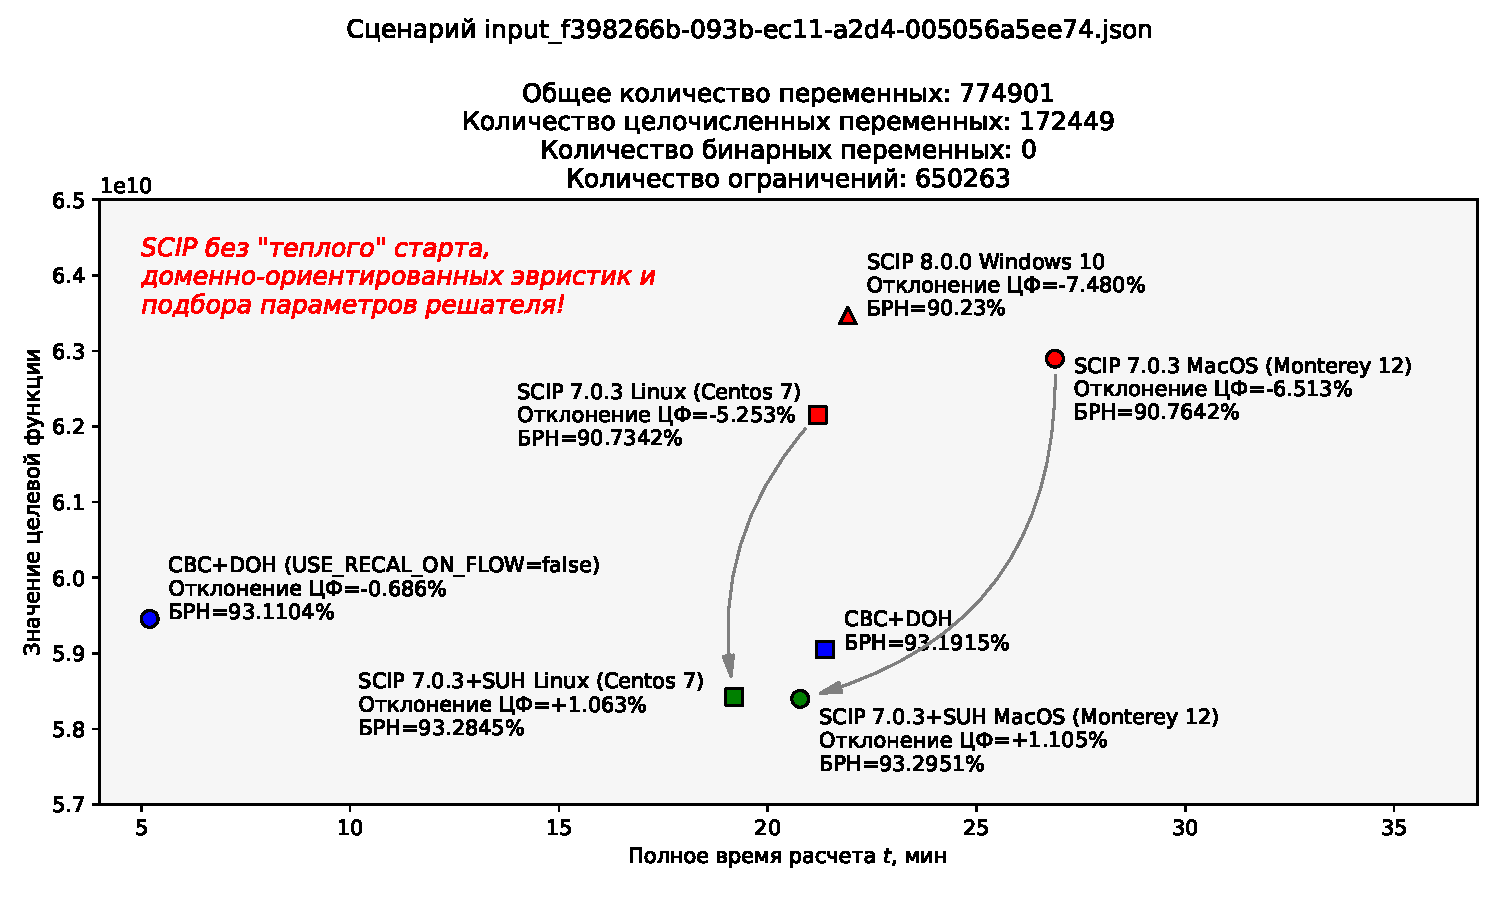
\includegraphics[scale=0.6]{figures/summary_f398266b.pdf}
	\caption{Сводка результатов анализа эффективности метаконфигурации SUH. \\Сценарий \texttt{f398266b} без бинарных переменных}\label{fig:summary_f398266b}
\end{figure}


\subsubsection{Сценарий \texttt{50197DF7} без бинарных переменных}

\textbf{Статистика}\vspace*{1mm}

Общее количество переменных: 718464

Количество целочисленных переменных: 159332

Количество бинарных переменных: 0

Количество ограничений: 595797

lp-файл: \url{https://disk.yandex.ru/d/KO_xj9dkgUdcog}

\vspace*{5mm}\textbf{Анализ решения}\vspace*{1mm}

Пул решений задачи был найден с помощью следующих первичных эвристик:
\begin{itemize}
	\item INTSHIFING,
	
	\item RENS.
\end{itemize}

Файл решения задачи (метаконфигурация SUH) доступен по ссылке \url{https://disk.yandex.ru/d/R4B1fkTx-nE3tg}

Файл статистической сводки (метаконфигурация SUH) доступен по ссылке \url{https://disk.yandex.ru/d/BLvUmZ43vtMFKg}

Файл решения задачи (метаконфигурация FZBIVSUHPB) доступен по ссылке \url{https://disk.yandex.ru/d/yMFLr-6mLfdPAw}

Файл статистической сводки (метаконфигурация FZBIVSUHPB) доступен по ссылке \url{https://disk.yandex.ru/d/XiRSvteL9xC4pg}

\vspace*{3mm}
\textbf{Вывод по сценарию}: описанная выше метаконфигурация SUH приводит к решению задачи, которое оказывается по отношению к результату на доменно-ориентированных эвристиках (\verb|USE_RECALCULATION_ON_FLOW=true|) для последнего решения из пула допустимых целочисленных решений (ОС Linux Centos 7) на 1.25\% лучше в смысле целевой функции и на 46.43\% -- в смысле временных издержек (\pic{fig:summary_50197df7}). 

Метаконфигурация FZBIVSUHPB (подробнее в разделе~\ref{sec:ikp_bins}) по отношению к тому же результату на доменно-ориентированных эвристиках дает решение задачи, которое на 1.191\% лучше в смысле целевой функции и на 82.13\% -- в смысле временных издержек (\tblref{tab:50197df7_wo_bins}).

Синим цветом обозначен выигрыш в процентах.

{
	%\rowcolors{2}{white}{lightgray!15}
	\begin{table}[!h]
		\centering
		\caption{Сводка результатов анализа эффективности \\метаконфигураций SUH и FZBIVSUHPB. Сценарий \texttt{50197df7} без бинарных переменных}
		\begin{tabular}{ p{2.5cm} p{3.3cm} p{3.4cm} }
			\emph{Способ} & \emph{Полное время расчета, мин} & \emph{Верхняя граница решения, $ \times 10^{10} $} \\
			\hline\hline\\[-3.5mm]
			{CBC+DOH} & 18.35 & $ 3.585532 $ \\
			\hline
			SCIP+SUH & 9.83 {\color{blue} $\ +46.43 $\%} & $ 3.540567 $ {\color{blue} $\ +1.252 $\%} \\
			\hline
			SCIP+FZB... & 3.28 {\color{blue} $\ +82.13 $\%} & $ 3.542843 $ {\color{blue} $\ +1.191 $\%} \\
		\end{tabular}\label{tab:50197df7_wo_bins}
	\end{table}
}

\begin{figure}[!h]
	\centering
	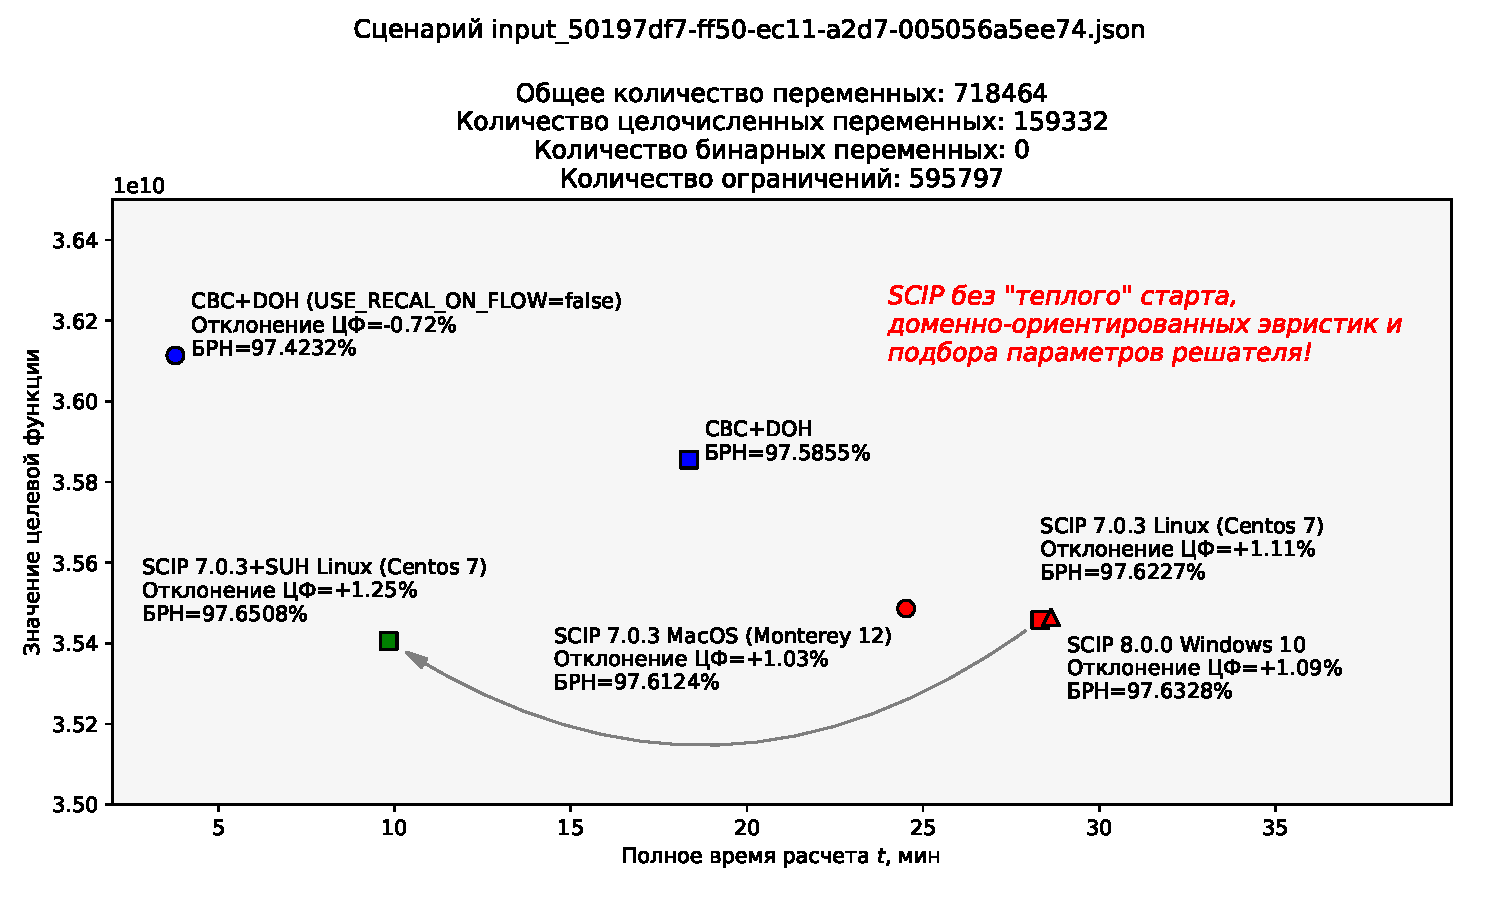
\includegraphics[scale=0.6]{figures/summary_50197df7.pdf}
	\caption{Сводка результатов анализа эффективности метаконфигурации SUH. \\Сценарий \texttt{50197df7} без бинарных переменных}\label{fig:summary_50197df7}
\end{figure}

\subsubsection{Сценарий \texttt{7FAC4231} без бинарных переменных}

\textbf{Статистика}\vspace*{1mm}

Общее количество переменных: 737585

Количество целочисленных переменных: 147789

Количество бинарных переменных: 0

Количество ограничений: 540018

lp-файл: \url{https://disk.yandex.ru/d/qiZAmraUNK1Peg}

\vspace*{5mm}\textbf{Анализ решения}\vspace*{1mm}

Пул решений задачи был найден с помощью следующих первичных эвристик:
\begin{itemize}
	\item INTSHIFING,
	
	\item RENS.
\end{itemize}

Файл решения задачи (метаконфигурация SUH) доступен по ссылке \url{https://disk.yandex.ru/d/20NeMuQ7NF_ccA}

Файл статистической сводки (метаконфигурация SUH) доступен по ссылке \url{https://disk.yandex.ru/d/QxE0HoREHzgHQQ}

Файл решения задачи (метаконфигурация FZBIVSUHPB) доступен по ссылке \url{https://disk.yandex.ru/d/FHZGj_Kyg8dDiw}

Файл статистической сводки (метаконфигурация FZBIVSUHPB) доступен по ссылке \url{https://disk.yandex.ru/d/8H1vw6zkQS7DAg}

\vspace*{3mm}
\textbf{Вывод по сценарию}: описанная выше метаконфигурация SUH приводит к решению задачи, которое оказывается по отношению к результату на доменно-ориентированных эвристиках (\verb|USE_RECALCULATION_ON_FLOW=true|) для последнего решения из пула допустимых целочисленных решений (ОС Linux Centos 7) на 5.22\% лучше в смысле целевой функции и на 27.10\% -- в смысле временных издержек (\pic{fig:summary_7fac4231}).

Метаконфигурация FZBIVSUHPB (подробнее в разделе~\ref{sec:ikp_bins}) по отношению к тому же результату на доменно-ориентированных эвристиках дает решение задачи, которое на 5.452\% лучше в смысле целевой функции и на 90.16\% -- в смысле временных издержек (\tblref{tab:7fac4231_wo_bins}).

Синим цветом обозначен выигрыш в процентах.

{
	%\rowcolors{2}{white}{lightgray!15}
	\begin{table}[!h]
		\centering
		\caption{Сводка результатов анализа эффективности \\метаконфигураций SUH и FZBIVSUHPB. Сценарий \texttt{7fac4231} без бинарных переменных}
		\begin{tabular}{ p{2.5cm} p{3.3cm} p{3.4cm} }
			\emph{Способ} & \emph{Полное время расчета, мин} & \emph{Верхняя граница решения, $ \times 10^{10} $} \\
			\hline\hline\\[-3.5mm]
			{CBC+DOH} & 16.05 & $ 1.087609 $ \\
			\hline
			SCIP+SUH & 11.67 {\color{blue} $\ +27.29 $\%} & $ 1.030866 $ {\color{blue} $\ +5.222 $\%} \\
			\hline
			SCIP+FZB... & 3.58 {\color{blue} $\ +77.69 $\%} & $ 1.028349 $ {\color{blue} $\ +5.452 $\%} \\
		\end{tabular}\label{tab:7fac4231_wo_bins}
	\end{table}
}

\begin{figure}[!h]
	\centering
	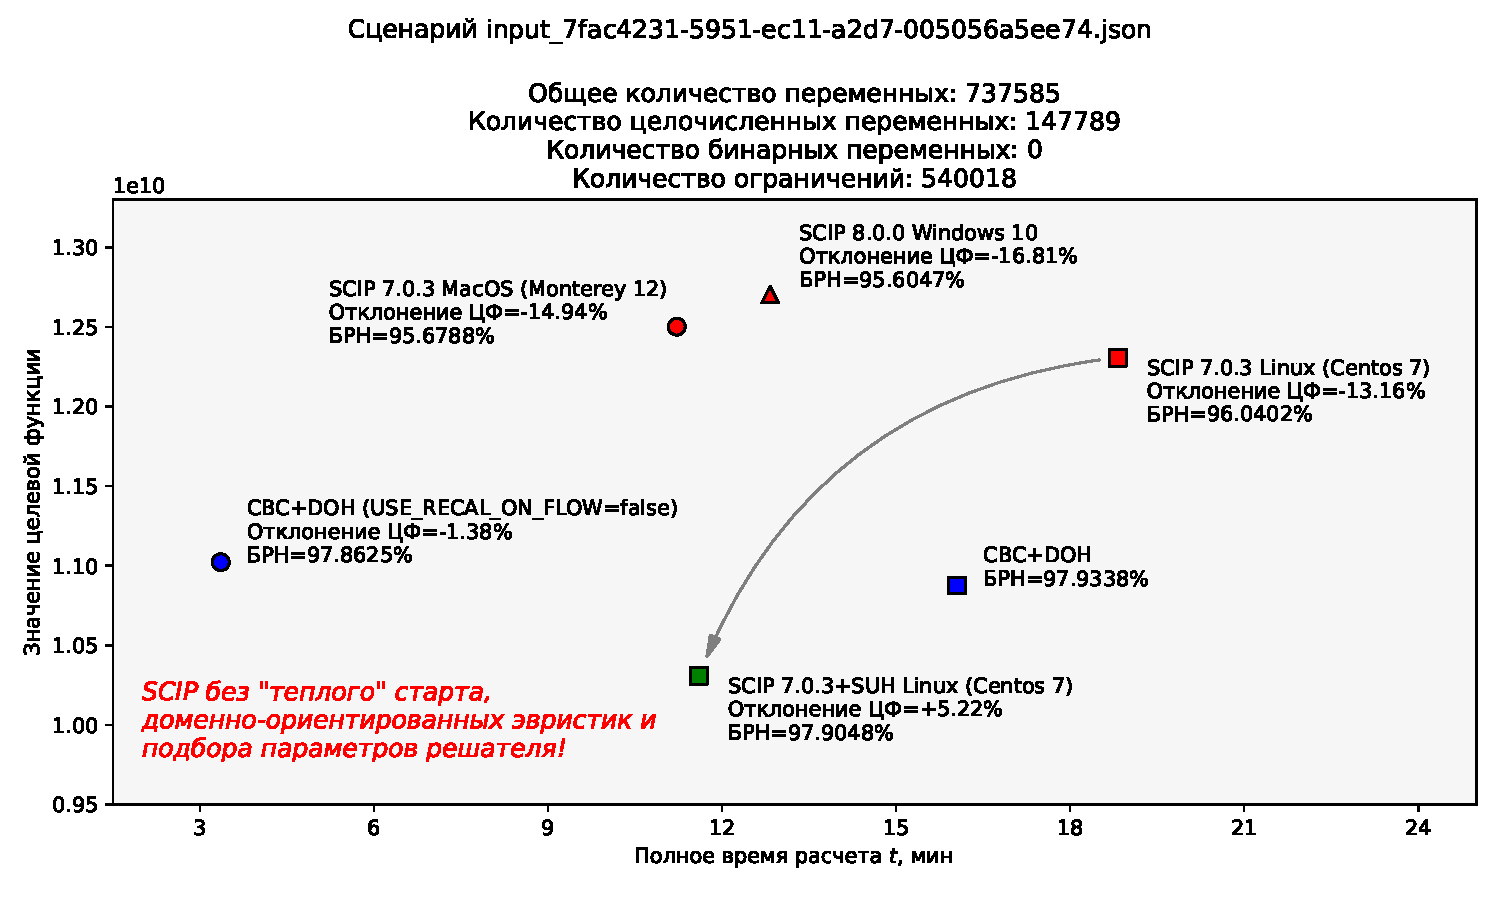
\includegraphics[scale=0.6]{figures/summary_7fac4231.pdf}
	\caption{Сводка результатов анализа эффективности метаконфигурации SUH. \\Сценарий \texttt{7fac4231} без бинарных переменных}\label{fig:summary_7fac4231}
\end{figure}

\subsubsection{Сценарий \texttt{CA485A55} без бинарных переменных}

\textbf{Статистика}\vspace*{1mm}

Общее количество переменных: 718601

Количество целочисленных переменных: 140858

Количество бинарных переменных: 0

Количество ограничений: 514229

lp-файл: \url{https://disk.yandex.ru/d/iSP6xrh4K_wHEQ}

\vspace*{5mm}\textbf{Анализ решения}\vspace*{1mm}

Пул решений задачи был найден с помощью следующих первичных эвристик:
\begin{itemize}
	\item INTSHIFING,
	
	\item RENS.
\end{itemize}

Файл решения задачи (метаконфигурация SUH) доступен по ссылке \url{https://disk.yandex.ru/d/_WzkmgoueNb2Bg}

Файл решения задачи (метаконфигурация FZBIVSUHPB) доступен по ссылке \url{https://disk.yandex.ru/d/sLUW5IxmpMBpcw}

Файл статистической сводки (метаконфигурация FZBIVSUHPB) доступен по ссылке \url{https://disk.yandex.ru/d/3Ls6QrAWVUMdZw}

\vspace*{3mm}
\textbf{Вывод по сценарию}: описанная выше метаконфигурация SUH приводит к решению задачи, которое оказывается по отношению к результату на доменно-ориентированных эвристиках (\verb|USE_RECALCULATION_ON_FLOW=true|) для последнего решения из пула допустимых целочисленных решений (ОС Linux Centos 7) на 0.683\% лучше в смысле целевой функции и на 46.48\% -- в смысле временных издержек (\pic{fig:summary_ca485a55}).

Метаконфигурация FZBIVSUHPB (подробнее в разделе~\ref{sec:ikp_bins}) по отношению к тому же результату на доменно-ориентированных эвристиках дает решение задачи, которое на 1.244\% лучше в смысле целевой функции и на 88.53\% -- в смысле временных издержек (\tblref{tab:ca485a55_wo_bins}).

Синим цветом обозначен выигрыш в процентах.

{
	%\rowcolors{2}{white}{lightgray!15}
	\begin{table}[!h]
		\centering
		\caption{Сводка результатов анализа эффективности \\метаконфигураций SUH и FZBIVSUHPB. Сценарий \texttt{ca485a55} без бинарных переменных}
		\begin{tabular}{ p{2.5cm} p{3.3cm} p{3.4cm} }
			\emph{Способ} & \emph{Полное время расчета, мин} & \emph{Верхняя граница решения, $ \times 10^{10} $} \\
			\hline\hline\\[-3.5mm]
			{CBC+DOH} & 20.05 & $ 4.597048 $ \\
			\hline
			SCIP+SUH & 10.73 {\color{blue} $\ +46.48 $\%} & $ 4.565579 $ {\color{blue} $\ +0.683 $\%} \\
			\hline
			SCIP+FZB... & 4.34 {\color{blue} $\ +78.35 $\%} & $ 4.539819 $ {\color{blue} $\ +1.244 $\%} \\
		\end{tabular}\label{tab:ca485a55_wo_bins}
	\end{table}
}

\begin{figure}[!h]
	\centering
	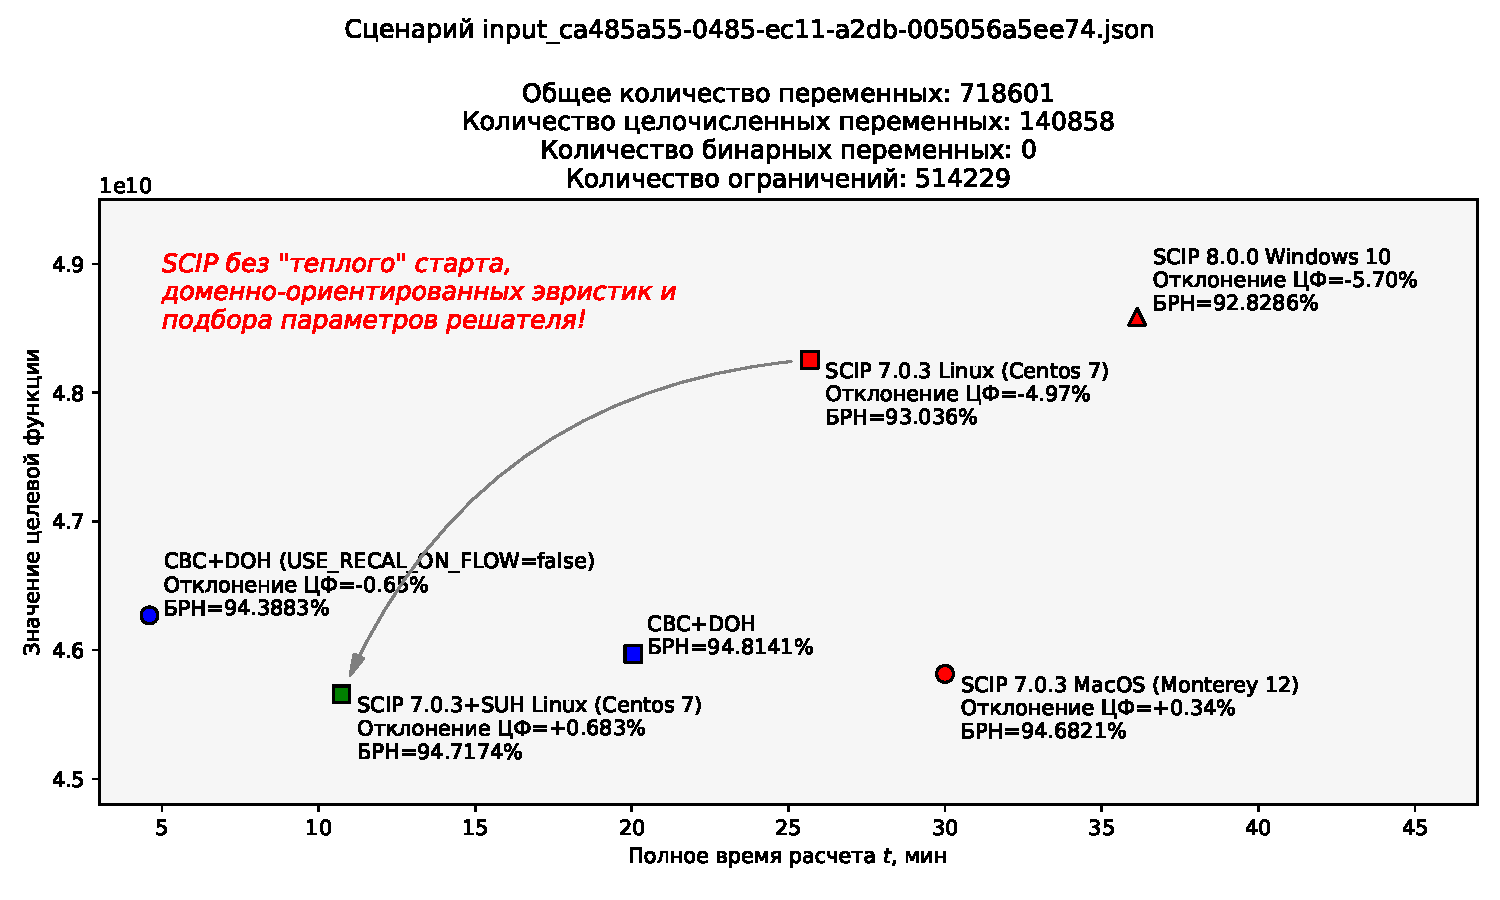
\includegraphics[scale=0.6]{figures/summary_ca485a55.pdf}
	\caption{Сводка результатов анализа эффективности метаконфигурации SUH. \\Сценарий \texttt{ca485a55} без бинарных переменных}\label{fig:summary_ca485a55}
\end{figure}

\subsubsection{Сценарий \texttt{276} без бинарных переменных}

\textbf{Статистика}\vspace*{1mm}

Общее количество переменных: 809224

Количество целочисленных переменных: 162562

Количество бинарных переменных: 0

Количество ограничений: 602190

lp-файл: \url{https://disk.yandex.ru/d/QaS5kd7VRZQ66A}

\vspace*{5mm}\textbf{Анализ решения}\vspace*{1mm}

Пул решений задачи был найден с помощью следующих первичных эвристик:
\begin{itemize}
	\item INTSHIFING,
	
	\item RENS.
\end{itemize}

Файл решения задачи (метаконфигурация SUH) доступен по ссылке \url{https://disk.yandex.ru/d/M2V88djiiGM5PA}

Файл решения задачи (метаконфигурация FZBIVSUHPB) доступен по ссылке \url{https://disk.yandex.ru/d/G0ustAVT6I9CeA}

Файл статистической сводки (метаконфигурация FZBIVSUHPB) доступен по ссылке \url{https://disk.yandex.ru/d/YBXB5GCECJiBIA}

\vspace*{3mm}
\textbf{Вывод по сценарию}: описанная выше метаконфигурация SUH приводит к решению задачи, которое оказывается по отношению к результату на доменно-ориентированных эвристиках (\verb|USE_RECALCULATION_ON_FLOW=true|) для последнего решения из пула допустимых целочисленных решений (ОС Linux Centos 7) на 3.67\% лучше в смысле целевой функции и на 51.56\% -- в смысле временных издержек (\pic{fig:summary_276}).

Метаконфигурация FZBIVSUHPB (подробнее в разделе~\ref{sec:ikp_bins}) по отношению к тому же результату на доменно-ориентированных эвристиках дает решение задачи, которое на 4.86\% лучше в смысле целевой функции и на 78.35\% -- в смысле временных издержек (\tblref{tab:276_wo_bins}).

Синим цветом обозначен выигрыш в процентах.

{
	%\rowcolors{2}{white}{lightgray!15}
	\begin{table}[!h]
		\centering
		\caption{Сводка результатов анализа эффективности \\метаконфигураций SUH и FZBIVSUHPB. Сценарий \texttt{276} без бинарных переменных}
		\begin{tabular}{ p{2.5cm} p{3.3cm} p{3.4cm} }
			\emph{Способ} & \emph{Полное время расчета, мин} & \emph{Верхняя граница решения, $ \times 10^{10} $} \\
			\hline\hline\\[-3.5mm]
			{CBC+DOH} & 29.87 & $ 1.430789 $ \\
			\hline
			SCIP+SUH & 14.47 {\color{blue} $\ +51.56 $\%} & $ 1.378299 $ {\color{blue} $\ +3.669 $\%} \\
			\hline
			SCIP+FZB... & 3.95 {\color{blue} $\ +78.35 $\%} & $ 1.361368 $ {\color{blue} $\ +4.857 $\%} \\
		\end{tabular}\label{tab:276_wo_bins}
	\end{table}
}


\begin{figure}[!h]
	\centering
	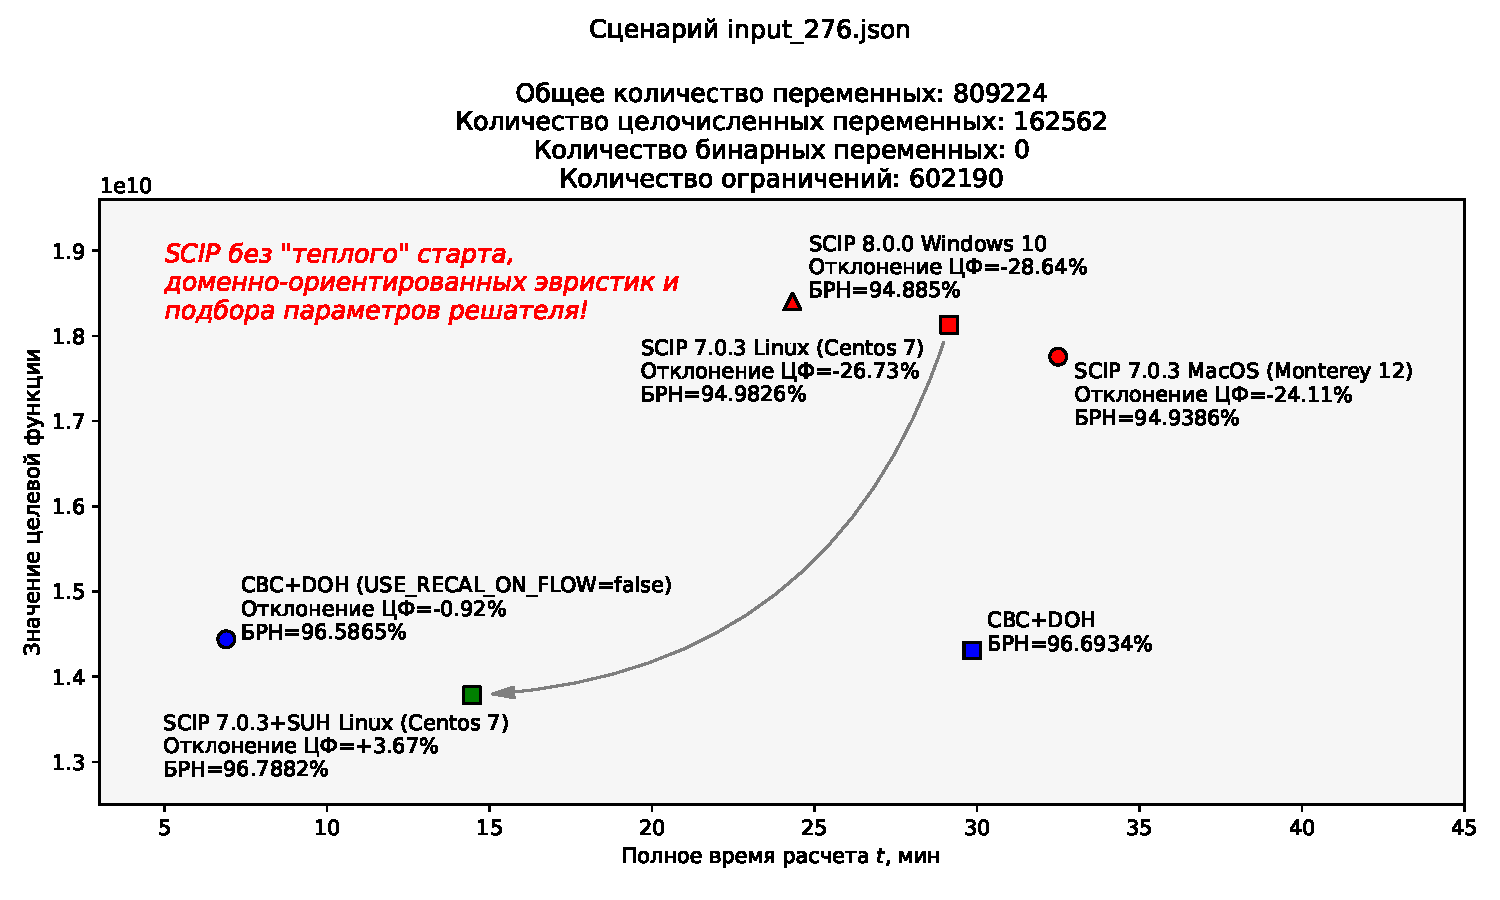
\includegraphics[scale=0.6]{figures/summary_276.pdf}
	\caption{Сводка результатов анализа эффективности метаконфигурации SUH. \\Сценарий \texttt{276} без бинарных переменных}\label{fig:summary_276}
\end{figure}

\subsubsection{Сценарий \texttt{337} без бинарных переменных}

\textbf{Статистика}\vspace*{1mm}

Общее количество переменных: 859075

Количество целочисленных переменных: 173622

Количество бинарных переменных: 0

Количество ограничений: 624327

lp-файл: \url{https://disk.yandex.ru/d/keyQLAagsD7Sbw}

\vspace*{5mm}\textbf{Анализ решения}\vspace*{1mm}

Пул решений задачи был найден с помощью следующих первичных эвристик:
\begin{itemize}
	\item INTSHIFING,
	
	\item RENS.
\end{itemize}

Файл решения задачи (метаконфигурация SUH) доступен по ссылке \url{https://disk.yandex.ru/d/ZUIEo3dDq77FjA}

Файл решения задачи (метаконфигурация FZBIVSUHPB) доступен по ссылке \url{https://disk.yandex.ru/d/0nUXIrIKuzqZlw}

Файл статистической сводки (метаконфигурация FZBIVSUHPB) доступен по ссылке \url{https://disk.yandex.ru/d/U0NCnMQN1akHUA}

\vspace*{3mm}
\textbf{Вывод по сценарию}: описанная выше метаконфигурация SUH приводит к решению задачи, которое оказывается по отношению к результату на доменно-ориентированных эвристиках (\verb|USE_RECALCULATION_ON_FLOW=true|) для последнего решения из пула допустимых целочисленных решений (ОС Linux Centos 7) на 22.12\% лучше в смысле целевой функции и на 18.32\% -- в смысле временных издержек (\pic{fig:summary_337}).

Метаконфигурация FZBIVSUHPB (подробнее в разделе~\ref{sec:ikp_bins}) по отношению к тому же результату на доменно-ориентированных эвристиках дает решение задачи, которое на 22.59\% лучше в смысле целевой функции и на 70.84\% -- в смысле временных издержек (\tblref{tab:337_wo_bins}).

Синим цветом обозначен выигрыш в процентах.

{
	%\rowcolors{2}{white}{lightgray!15}
	\begin{table}[!h]
		\centering
		\caption{Сводка результатов анализа эффективности \\метаконфигураций SUH и FZBIVSUHPB. Сценарий \texttt{337} без бинарных переменных}
		\begin{tabular}{ p{2.5cm} p{3.3cm} p{3.4cm} }
			\emph{Способ} & \emph{Полное время расчета, мин} & \emph{Верхняя граница решения, $ \times 10^{10} $} \\
			\hline\hline\\[-3.5mm]
			{CBC+DOH} & 20.85 & $ 3.825042 $ \\
			\hline
			SCIP+SUH & 17.03 {\color{blue} $\ +18.32 $\%} & $ 2.978782 $ {\color{blue} $\ +22.123 $\%} \\
			\hline
			SCIP+FZB... & 6.08 {\color{blue} $\ +70.84 $\%} & $ 2.961019 $ {\color{blue} $\ +22.588 $\%} \\
		\end{tabular}\label{tab:337_wo_bins}
	\end{table}
}


\begin{figure}[!h]
	\centering
	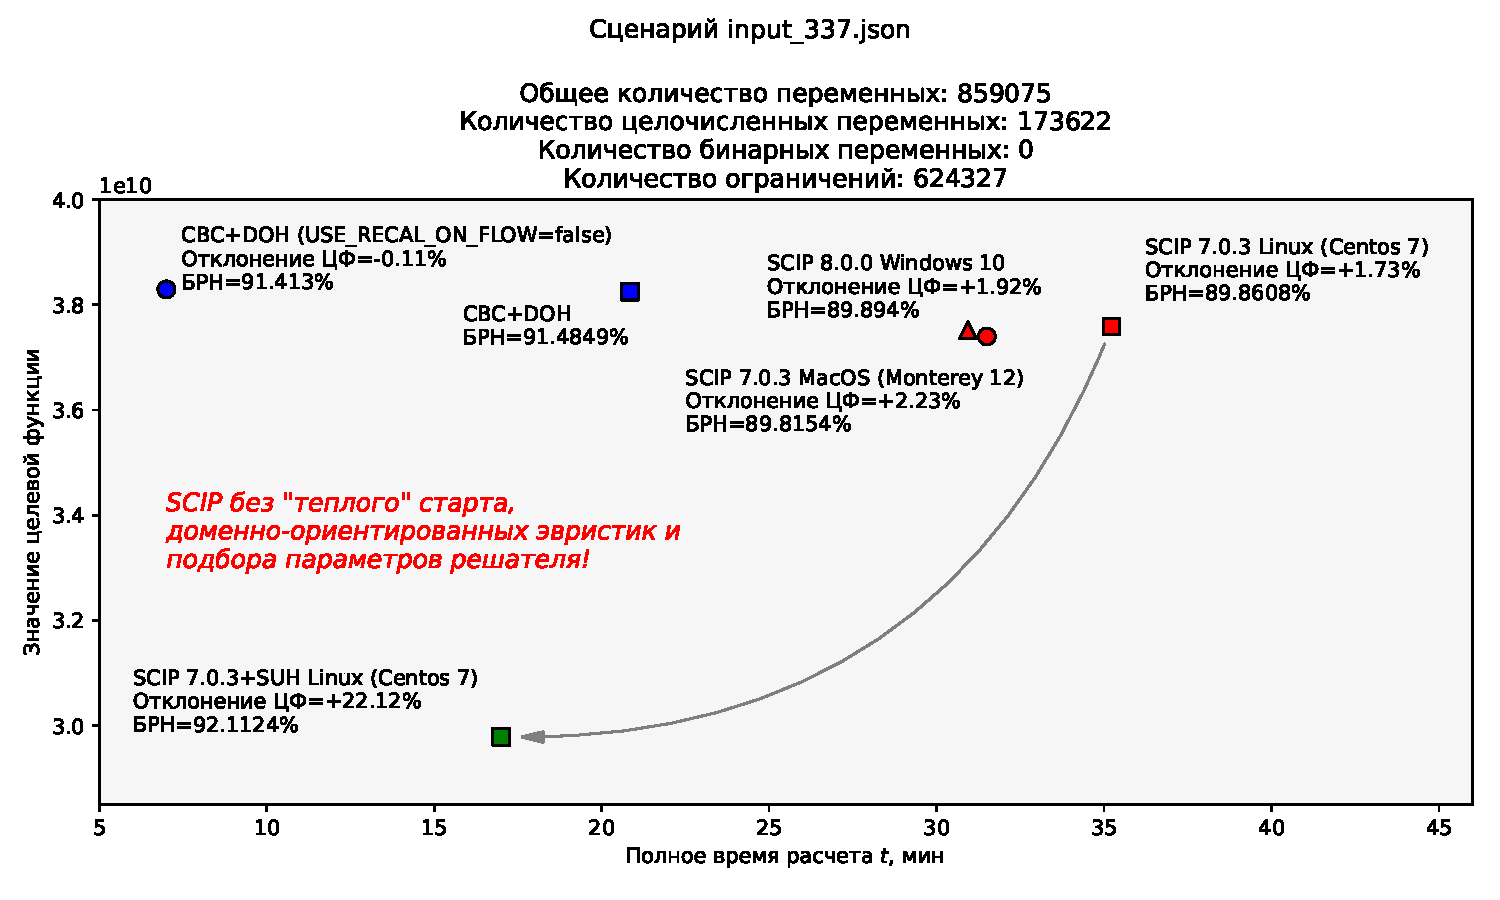
\includegraphics[scale=0.6]{figures/summary_337.pdf}
	\caption{Сводка результатов анализа эффективности метаконфигурации SUH. \\Сценарий \texttt{337} без бинарных переменных}\label{fig:summary_337}
\end{figure}

\subsubsection{Сценарий \texttt{13D686AB} без бинарных переменных}

\textbf{Статистика}\vspace*{1mm}

Общее количество переменных: 786020

Количество целочисленных переменных: 168857

Количество бинарных переменных: 0

Количество ограничений: 598414

lp-файл: \url{https://disk.yandex.ru/d/3KkYKzNl3PjGdg}

Пул решений задачи был найден с помощью следующих первичных эвристик:
\begin{itemize}
	\item INTSHIFING,
	
	\item RENS.
\end{itemize}

Файл решения задачи (метаконфигурация SUH) доступен по ссылке \url{https://disk.yandex.ru/d/EXylMeX6Ytz4tg}

Файл решения задачи (метаконфигурация FZBIVSUHPB) доступен по ссылке \url{https://disk.yandex.ru/d/dXUMVbSWRbqeDQ}

Файл статистической сводки (метаконфигурация FZBIVSUHPB) доступен по ссылке \url{https://disk.yandex.ru/d/Knavj89muxGw-w}

\vspace*{3mm}
\textbf{Вывод по сценарию}: описанная выше метаконфигурация SUH приводит к решению задачи, которое оказывается по отношению к результату на доменно-ориентированных эвристиках (\verb|USE_RECALCULATION_ON_FLOW=true|) для последнего решения из пула допустимых целочисленных решений (ОС Linux Centos 7) на 9.40\% лучше в смысле целевой функции и на 33.03\% -- в смысле временных издержек (\pic{fig:summary_13d686ab}).

Метаконфигурация FZBIVSUHPB (подробнее в разделе~\ref{sec:ikp_bins}) по отношению к тому же результату на доменно-ориентированных эвристиках дает решение задачи, которое на 10.44\% лучше в смысле целевой функции и на  75.82\% -- в смысле временных издержек (\tblref{tab:13d686ab_wo_bins}).

Синим цветом обозначен выигрыш в процентах.

{
	%\rowcolors{2}{white}{lightgray!15}
	\begin{table}[!h]
		\centering
		\caption{Сводка результатов анализа эффективности \\метаконфигураций SUH и FZBIVSUHPB. Сценарий \texttt{13d686ab} без бинарных переменных}
		\begin{tabular}{ p{2.5cm} p{3.3cm} p{3.4cm} }
			\emph{Способ} & \emph{Полное время расчета, мин} & \emph{Верхняя граница решения, $ \times 10^{9} $} \\
			\hline\hline\\[-3.5mm]
			{CBC+DOH} & 28.82 & $ 8.774743 $ \\
			\hline
			SCIP+SUH & 19.30 {\color{blue} $\ +33.03 $\%} & $ 7.949568 $ {\color{blue} $\ +9.403 $\%} \\
			\hline
			SCIP+FZB... & 6.97 {\color{blue} $\ +75.82 $\%} & $ 7.858548 $ {\color{blue} $\ +10.441 $\%} \\
		\end{tabular}\label{tab:13d686ab_wo_bins}
	\end{table}
}

\begin{figure}[!h]
	\centering
	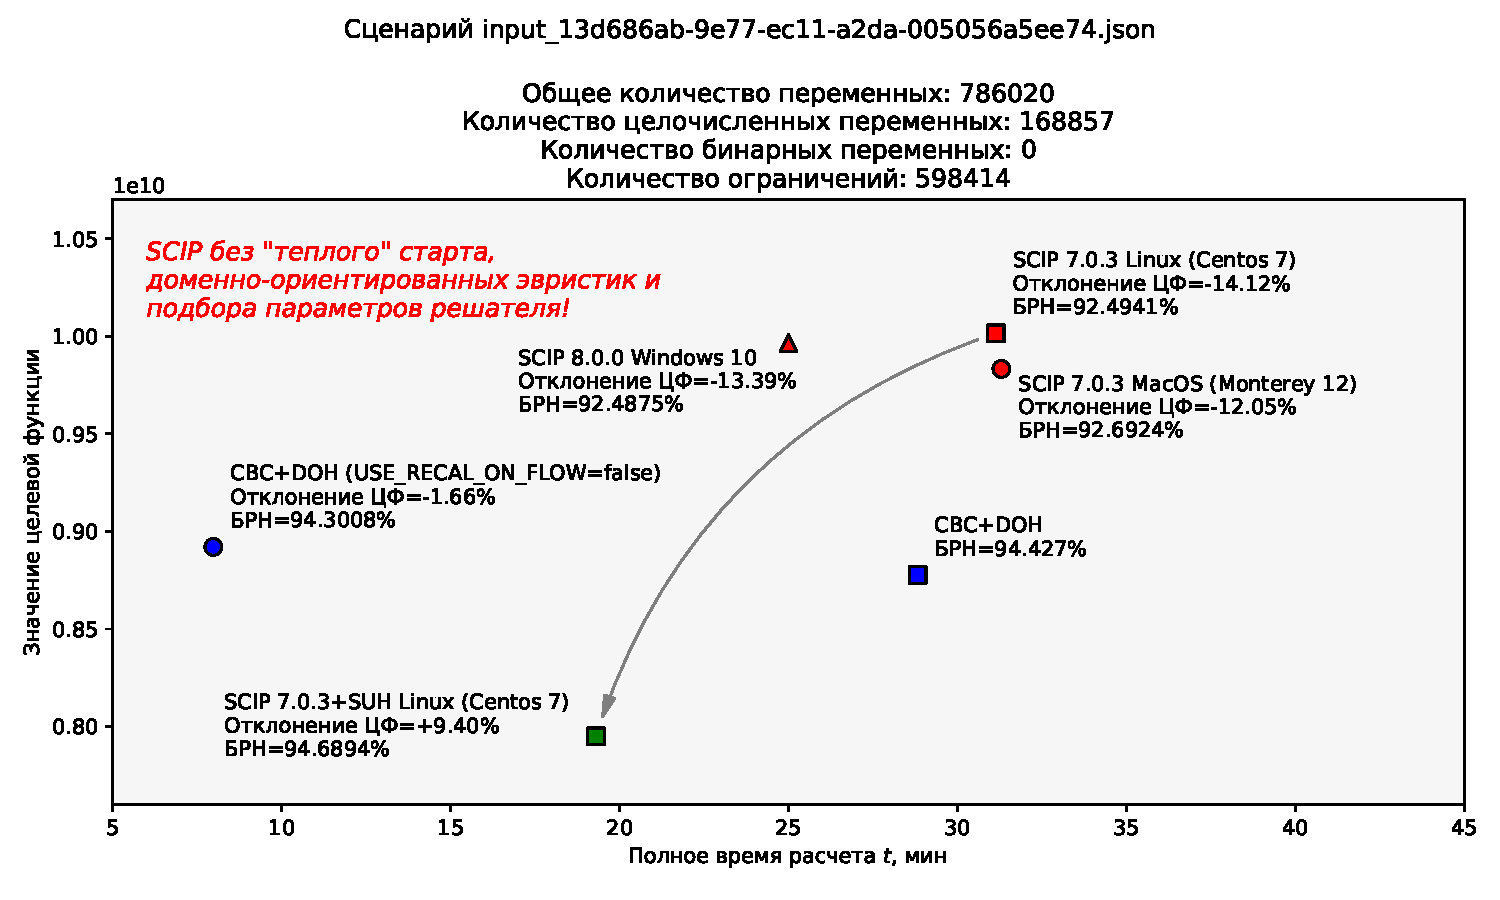
\includegraphics[scale=0.6]{figures/summary_13d686ab.pdf}
	\caption{Сводка результатов анализа эффективности метаконфигурации SUH. \\Сценарий \texttt{13d686ab} без бинарных переменных}\label{fig:summary_13d686ab}
\end{figure}

\subsubsection{Сценарий \texttt{A78CBEAD} без бинарных переменных}

\textbf{Статистика}\vspace*{1mm}

Общее количество переменных: 795400

Количество целочисленных переменных: 180160

Количество бинарных переменных: 0

Количество ограничений: 658339

lp-файл: \url{https://disk.yandex.ru/d/vTPPa1H3VFD7tA}

Пул решений задачи был найден с помощью следующих первичных эвристик:
\begin{itemize}
	\item INTSHIFING,
	
	\item RENS.
\end{itemize}

Файл решения задачи (метаконфигурация SUH) доступен по ссылке \url{https://disk.yandex.ru/d/fARVcHb66ToHxQ}

Файл решения задачи (метаконфигурация FZBIVSUHPB) доступен по ссылке \url{https://disk.yandex.ru/d/OXC17sTce8feHQ}

Файл статистической сводки (метаконфигурация FZBIVSUHPB) доступен по ссылке \url{https://disk.yandex.ru/d/vn1K834mY5MEng}

\vspace*{3mm}
\textbf{Вывод по сценарию}: описанная выше метаконфигурация SUH приводит к решению задачи, которое оказывается по отношению к результату на доменно-ориентированных эвристиках (\verb|USE_RECALCULATION_ON_FLOW=true|) для последнего решения из пула допустимых целочисленных решений (ОС Linux Centos 7) на 1.57\% лучше в смысле целевой функции и на 23.30\% -- в смысле временных издержек (\pic{fig:summary_a78cbead}).

Метаконфигурация FZBIVSUHPB (подробнее в разделе~\ref{sec:ikp_bins}) по отношению к тому же результату на доменно-ориентированных эвристиках дает решение задачи, которое на 1.39\% лучше в смысле целевой функции и на  81.04\% -- в смысле временных издержек (\tblref{tab:a78cbead_wo_bins}).

Синим цветом обозначен выигрыш в процентах.

{
	%\rowcolors{2}{white}{lightgray!15}
	\begin{table}[!h]
		\centering
		\caption{Сводка результатов анализа эффективности \\метаконфигураций SUH и FZBIVSUHPB. Сценарий \texttt{a78cbead} без бинарных переменных}
		\begin{tabular}{ p{2.5cm} p{3.3cm} p{3.4cm} }
			\emph{Способ} & \emph{Полное время расчета, мин} & \emph{Верхняя граница решения, $ \times 10^{10} $} \\
			\hline\hline\\[-3.5mm]
			{CBC+DOH} & 26.05& $ 3.801546 $ \\
			\hline
			SCIP+SUH & 19.98 {\color{blue} $\ +23.30 $\%} & $ 3.741685 $ {\color{blue} $\ +1.576 $\%} \\
			\hline
			SCIP+FZB... & 4.94 {\color{blue} $\ +81.04 $\%} & $ 3.748890 $ {\color{blue} $\ +1.386 $\%} \\
		\end{tabular}\label{tab:a78cbead_wo_bins}
	\end{table}
}

\begin{figure}[!h]
	\centering
	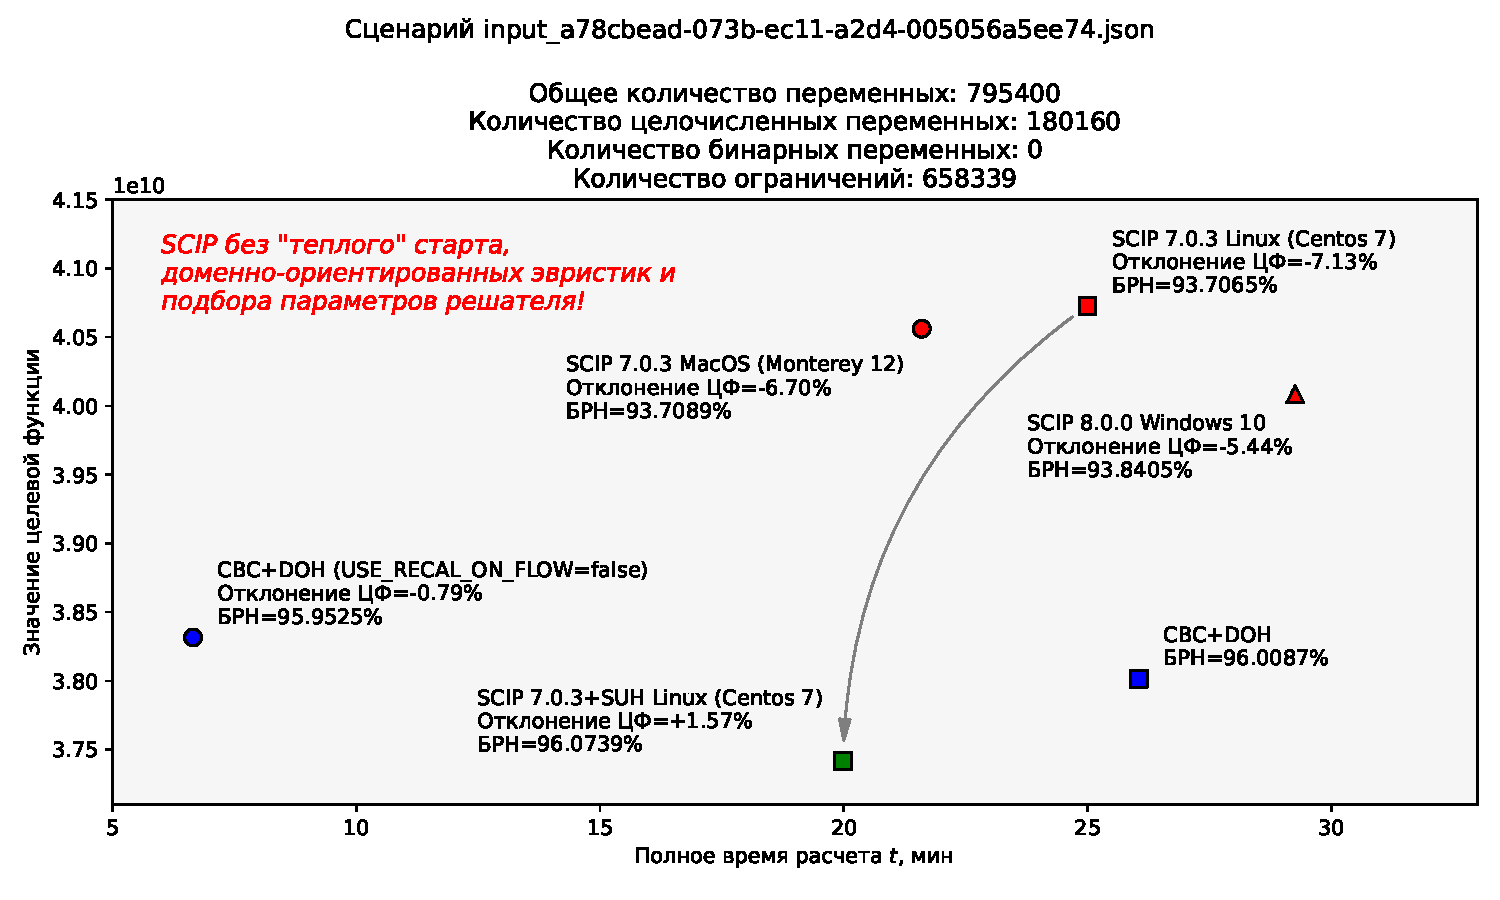
\includegraphics[scale=0.6]{figures/summary_a78cbead.pdf}
	\caption{Сводка результатов анализа эффективности метаконфигурации SUH. \\Сценарий \texttt{a78cbead} без бинарных переменных}\label{fig:summary_a78cbead}
\end{figure}


\subsection{Общие замечания по процедуре поиска решения на сценариях \emph{с} бинарными переменными}\label{sec:ikp_bins}

На ранних стадиях изучения проблемы высокоразмерных сценариев с бинарными переменными, поиск решения осуществлялся в семь шагов:
\begin{enumerate}
	\item  Подавить подгруппу первичных эвристик низкой эффективности (см. раздел ~\ref{sec:suh}),
	
	\item При разрешении конфликтов и ветвлении\footnote{К сожалению, на сценариях группы ИКП с бинарными переменными решателю SCIP не удается найти решение в корне дерева} отдавать предпочтение бинарным переменным,
	
	\item Найти релаксированное решение задачи,
	
	\item Подобрать порог бинаризации на релаксированном решении для бинарных переменных (см. раздел~\ref{sec:find_bin_thresh}),
	
	\item Зафиксировать \emph{нулевые} 0-bin и \emph{единичные} 1-bin \emph{бинарные переменные}; подать фиксацию решателю,
	
	\item В решении, найденном на предыдущей итерации, зафиксировать \emph{нулевые целочисленные} 0-int и \emph{единичные бинарные} 1-bin \emph{переменные}; полученную фиксацию подать на вход решателю,
	
	\item В решении, полученном на предыдущей итерации, зафиксировать \emph{нулевые бинарные} 0-bin и \emph{целочисленные} 0-int  \emph{переменные}; фиксацию подать на вход решателю.
\end{enumerate}

Процедура поиска оказалась чувствительной к параметру \texttt{autorestartnodes}. Графическая интерпретация результатов вычислительных экспериментов с разверткой процедуры поиска верхней границы решения во времени приведена на рис.~\ref{fig:a78cbead_autorestartnodes_1_2_phase}, \ref{fig:a78cbead_autorestartnodes_3_phase}, \ref{fig:50197df7_autorestartnodes} и \ref{fig:7fac4231_autorestartnodes}.

Позже описанную процедуру удалось упростить и свести к следующей \emph{метаконфигурации} {FZBIVSUHPB} (Fixed Zero Binary and Integer Variables, Suppress Useless Heuristics, Prefer Binary):
\begin{enumerate}
	\item Подавить подгруппу первичных эвристик низкой эффективности,
	
	\item При разрешении конфликтов и ветвлении отдавать предпочтение \emph{бинарным} переменным,
	
	\item Зафиксировать \emph{нулевые бинарные} 0-bin и \emph{нулевые целочисленные} 0-int  \emph{переменные} в релаксированном решении (см. раздел~\ref{sec:bin_int_relax_fix}).
\end{enumerate}

Конфигурация решателя SCIP для всех сценариев группы ИКП (с бинарными переменными) имеет вид
\begin{lstlisting}[
	title = {\sffamily scip.set. Сценарии группы ИКП с бинарными переменными},
	style = bash,
	numbers = none,
	]
# критерии останова и перезапуска
limits/time = 7200
limits/autorestartnodes = -1
limits/gap = 0.02  # решение останавливается при зазоре <= 2%

# управление стратегиями анализа конфликтов и ветвления
conflict/preferbinary = True
branching/preferbinary = True

# подавление подгруппы первичных эвристик низкой эффективности
heuristics/farkasdiving/freq = -1
heuristics/feaspump/freq = -1
heuristics/randrounding/freq = -1
heuristics/shiftandpropagate/freq = -1
heuristics/shifting/freq = -1
\end{lstlisting}

Все эксперименты проводились на виртуальной машине Linux (Centos 7) Intel Core™ i7 (8~CPUs), 3.6GHz, RAM 16Gb.

Сводка результатов вычислительных экспериментов доступна по ссылке \url{https://docs.google.com/document/d/1V9fZLT9cXkbVQ5BvMCwzKrAiASZ2v4-01Z68jVBZUBU/edit?usp=sharing}.

Кодовая база решения доступна по ссылке \url{https://gitdp.zyfra.com/ds_and_math_users/ml-dl-in-operations-reaseearches.git}

\subsubsection{Сценарий \texttt{A78CBEAD} с бинарными переменными}

\textbf{Статистика}\vspace*{1mm}

Общее количество переменных: 797818

Количество целочисленных переменных: 180160

Количество бинарных переменных: 2418

Количество ограничений: 663175

lp-файл: \url{https://disk.yandex.ru/d/JbT3KR5Yi1ZomQ}

\vspace*{5mm}\textbf{Анализ решения}\vspace*{1mm}

Пул решений задачи был найден с помощью следующих первичных эвристик:
\begin{itemize}
	\item DISTRIBUTIOINDIVING,
	
	\item ONEOPT,
	
	\item GINS.
\end{itemize}

Фргамент лога сессии SCIP
\begin{lstlisting}[
style = bash,
numbers = none
]
...
 time | node  | left  |LP iter|LP it/n|mem/heur|mdpt |vars |cons |rows |cuts |sepa|confs|strbr|  dualbound   | primalbound  |  gap   | compl. 
d1790s|  1881 |  1668 |  1010k| 296.9 |distribu|  93 |  50k|  43k|  43k|   0 |  1 | 385 |3585 | 3.757279e+10 | 3.894342e+10 |   3.65%|   7.70%
d1790s|  1881 |  1668 |  1010k| 296.9 |distribu|  93 |  50k|  43k|  43k|   0 |  1 | 385 |3585 | 3.757279e+10 | 3.894341e+10 |   3.65%|   7.70%
i1792s|  1882 |  1667 |  1011k| 297.0 |  oneopt|  93 |  50k|  43k|  43k|8612 |  0 | 385 |3585 | 3.757279e+10 | 3.893993e+10 |   3.64%|   7.70%
1796s|  1900 |  1687 |  1016k| 297.0 |  3669M |  93 |  50k|  43k|  43k|8644 |  1 | 387 |3585 | 3.757279e+10 | 3.893993e+10 |   3.64%|   2.82%
L1902s|  1982 |  1769 |  1090k| 313.4 |    gins|  93 |  50k|  43k|  43k|8935 |  1 | 398 |3590 | 3.757279e+10 | 3.875897e+10 |   3.16%|   2.83%
L1912s|  1982 |  1769 |  1090k| 313.4 |    gins|  93 |  50k|  43k|  43k|8935 |  1 | 398 |3590 | 3.757279e+10 | 3.864257e+10 |   2.85%|   2.83%
i1920s|  1982 |  1769 |  1099k| 316.2 |  oneopt|  93 |  50k|  43k|  43k|8935 |  1 | 398 |3590 | 3.757279e+10 | 3.864241e+10 |   2.85%|   2.83%
1954s|  2000 |  1787 |  1133k| 325.5 |  3731M |  93 |  50k|  43k|  43k|9004 |  1 | 398 |3591 | 3.757279e+10 | 3.864241e+10 |   2.85%|   2.83%
\end{lstlisting}

Файл решения задачи доступен по ссылке \url{https://disk.yandex.ru/d/6FPE-S5VupA6iw}

Файл статистической сводки доступен по ссылке \url{https://disk.yandex.ru/d/9G-v54ywEK1TJA}

\vspace*{3mm}
\textbf{Вывод по сценарию}: описанная выше метаконфигурация приводит к решению задачи, которое оказывается по отношению к результату на доменно-ориентированных эвристиках для последнего решения из пула допустимых целочисленных решений на 2.46\% лучше в смысле целевой функции и на 19.64\% -- в смысле временных издержек (\tblref{tab:a78cbead}).

В \tblref{tab:a78cbead}  через SCIP+MC~$ (a) $ обозначается решение, построенное на метаконфигурации SCIP, отвечающее \emph{первому} допустимому целочисленному решению, верхняя граница которого не превышает верхнюю границу решения на доменно-ориентированных эвристиках, а через SCIP+MC~$ (b) $ -- решение, отвечающее \emph{последнему} допустимому целочисленному решению в наборе полученных.

Синим цветом обозначен выигрыш в процентах.

{
%\rowcolors{2}{white}{lightgray!15}
\begin{table}[!h]
	\centering
	\caption{Сводка результатов анализа эффективности\\метаконфигурации FZBIVSUHPB. Сценарий \texttt{a78cbead} с бинарными переменными}
	\begin{tabular}{ p{2.5cm} p{3.3cm} p{3.4cm} }
		\emph{Способ} & \emph{Полное время расчета, мин} & \emph{Верхняя граница решения, $ \times 10^{10} $} \\
		\hline\hline\\[-3.5mm]
		{CBC+DOH} & 39.82 & $ 3.961502 $ \\
		\hline
		SCIP+MC ($ a $) & 29.83 {\color{blue} $\ +25.09 $\%} & $ 3.894342 $ {\color{blue} $\ +1.70 $\%} \\
		\hline
		SCIP+MC ($ b $) & 32.00 {\color{blue} $\ +19.64 $\%} & $ 3.864241 $ {\color{blue} $\ +2.46 $\%} \\
	\end{tabular}\label{tab:a78cbead}
\end{table}
}

\subsubsection{Сценарий \texttt{7FAC4231} с бинарными переменными}

\textbf{Статистика}\vspace*{1mm}

Общее количество переменных: 740251

Количество целочисленных переменных: 147789

Количество бинарных переменных: 2666

Количество ограничений: 545350

lp-файл: \url{https://disk.yandex.ru/d/3NbbjfLW5zhejQ}

\vspace*{5mm}\textbf{Анализ решения}\vspace*{1mm}

Пул решений задачи был найден с помощью следующих первичных эвристик:
\begin{itemize}
	\item INTSHIFTING,
	
	\item ONEOPT,
	
	\item GINS,
	
	\item CROSSOVER,
	
	\item ALNS.
\end{itemize}

Фрагмент лога сессии SCIP
\begin{lstlisting}[
style = bash,
numbers = none
]
...
 time | node  | left  |LP iter|LP it/n|mem/heur|mdpt |vars |cons |rows |cuts |sepa|confs|strbr|  dualbound   | primalbound  |  gap   | compl. 
r 454s|   372 |   341 | 91171 | 102.3 |intshift| 309 |  41k|  33k|  34k|2788 |  5 |  57 |3711 | 1.053077e+10 | 1.309195e+10 |  24.32%|   0.78%
i 454s|   373 |   340 | 91171 | 102.0 |  oneopt| 309 |  41k|  33k|  34k|2788 |  0 |  57 |3711 | 1.053077e+10 | 1.308634e+10 |  24.27%|   0.78%
463s|   400 |   369 | 93623 | 101.3 |  2493M | 309 |  41k|  33k|  34k|2950 |  1 |  57 |3761 | 1.053077e+10 | 1.308634e+10 |  24.27%|   0.29%
L 507s|   473 |   442 |106991 | 113.9 |    gins| 309 |  41k|  33k|  34k|3084 |  1 |  57 |3813 | 1.053077e+10 | 1.297515e+10 |  23.21%|   0.29%
L 512s|   473 |   442 |106991 | 113.9 |    gins| 309 |  41k|  33k|  34k|3084 |  1 |  57 |3813 | 1.053077e+10 | 1.292548e+10 |  22.74%|   0.29%
L 522s|   473 |   442 |106991 | 113.9 |    gins| 309 |  41k|  33k|  34k|3084 |  1 |  57 |3813 | 1.053077e+10 | 1.289283e+10 |  22.43%|   0.29%
L 525s|   473 |   442 |106991 | 113.9 |    gins| 309 |  41k|  33k|  34k|3084 |  1 |  57 |3813 | 1.053077e+10 | 1.286340e+10 |  22.15%|   0.29%
i 529s|   473 |   442 |112279 | 125.1 |  oneopt| 309 |  41k|  33k|  34k|3084 |  1 |  57 |3813 | 1.053077e+10 | 1.285668e+10 |  22.09%|   0.29%
r 531s|   474 |   443 |120630 | 142.5 |intshift| 309 |  41k|  33k|  34k|3084 |  1 |  58 |3813 | 1.053077e+10 | 1.197786e+10 |  13.74%|   0.29%
i 532s|   474 |   373 |124926 | 151.6 |  oneopt| 309 |  41k|  33k|  34k|3084 |  1 |  58 |3813 | 1.053077e+10 | 1.197230e+10 |  13.69%|   0.29%
536s|   500 |   399 |126496 | 146.9 |  2579M | 309 |  41k|  33k|  34k|3181 |  1 |  58 |3822 | 1.053077e+10 | 1.197230e+10 |  13.69%|   0.29%
567s|   600 |   499 |158520 | 175.8 |  2613M | 309 |  41k|  33k|  34k|3641 |  1 |  60 |3933 | 1.053095e+10 | 1.197230e+10 |  13.69%|   0.29%
L 739s|   659 |   554 |189783 | 207.6 |    gins| 309 |  41k|  33k|  34k|4060 |  1 |  62 |3978 | 1.053095e+10 | 1.191898e+10 |  13.18%|   0.29%
i 741s|   660 |   555 |198453 | 220.4 |  oneopt| 309 |  41k|  33k|  34k|4060 |  1 |  62 |3981 | 1.053095e+10 | 1.191889e+10 |  13.18%|   0.30%
794s|   700 |   595 |236166 | 261.7 |  2689M | 309 |  41k|  33k|  34k|4418 |  1 |  62 |4010 | 1.053095e+10 | 1.191889e+10 |  13.18%|   0.32%
836s|   800 |   695 |277232 | 280.4 |  2728M | 309 |  41k|  33k|  34k|4757 |  1 |  64 |4027 | 1.053219e+10 | 1.191889e+10 |  13.17%|   0.32%
L 967s|   860 |   693 |295017 | 281.5 |crossove| 309 |  41k|  33k|  34k|5000 |  1 |  64 |4059 | 1.053219e+10 | 1.154287e+10 |   9.60%|   0.32%
i 968s|   860 |   693 |300734 | 288.1 |  oneopt| 309 |  41k|  33k|  34k|5000 |  1 |  64 |4059 | 1.053219e+10 | 1.154284e+10 |   9.60%|   0.32%
990s|   900 |   733 |312921 | 288.9 |  2793M | 309 |  41k|  33k|  34k|5288 |  1 |  64 |4139 | 1.053219e+10 | 1.154284e+10 |   9.60%|   0.33%
1042s|  1000 |   823 |346085 | 293.2 |  2816M | 309 |  41k|  33k|  34k|5725 |  1 |  65 |4281 | 1.053219e+10 | 1.154284e+10 |   9.60%|   0.33%
L1083s|  1003 |   826 |347173 | 293.4 |    alns| 309 |  41k|  33k|  34k|5747 |  2 |  65 |4284 | 1.053219e+10 | 1.153273e+10 |   9.50%|   0.33%
i1084s|  1004 |   827 |352908 | 298.8 |  oneopt| 309 |  41k|  33k|  34k|5747 |  1 |  65 |4284 | 1.053219e+10 | 1.118743e+10 |   6.22%|   0.33%
1113s|  1100 |   699 |373504 | 291.4 |  2860M | 309 |  41k|  33k|  34k|6055 |  3 |  65 |4323 | 1.053219e+10 | 1.118743e+10 |   6.22%|   0.44%
1140s|     1 |     0 |419115 |     - |  3039M |   0 |  41k|  34k|  34k|   0 |  0 |  65 |4323 | 1.053219e+10 | 1.118743e+10 |   6.22%| unknown
\end{lstlisting}

Файл решения задачи доступен по ссылке \url{https://disk.yandex.ru/d/TmA6hqFV87eGTg}

Файл статистической сводки доступен по ссылке \url{https://disk.yandex.ru/d/CsGV_oal4OTxOQ}

\vspace*{3mm}
\textbf{Вывод по сценарию}: описанная выше метаконфигурация приводит к решению задачи, которое оказывается по отношению к результату на доменно-ориентированных эвристиках для последнего решения из пула допустимых целочисленных решений на 3.38\% лучше в смысле целевой функции и на 33.07\% -- в смысле временных издержек (\tblref{tab:7fac4231}).

В \tblref{tab:7fac4231}  через SCIP+MC~$ (a) $ обозначается решение, построенное на метаконфигурации SCIP, отвечающее \emph{первому} допустимому целочисленному решению, верхняя граница которого не превышает верхнюю границу решения на доменно-ориентированных эвристиках, а через SCIP+MC~$ (b) $ -- решение, отвечающее \emph{последнему} допустимому целочисленному решению в наборе полученных.

Синим цветом обозначен выигрыш в процентах.

{
	%\rowcolors{2}{white}{lightgray!15}
	\begin{table}[!h]
		\centering
		\caption{Сводка результатов анализа эффективности\\метаконфигурации FZBIVSUHPB. Сценарий \texttt{7fac4231} с бинарными переменными}
		\begin{tabular}{ p{2.5cm} p{3.3cm} p{3.4cm} }
			\emph{Способ} & \emph{Полное время расчета, мин} & \emph{Верхняя граница решения, $ \times 10^{10} $} \\
			\hline\hline\\[-3.5mm]
			{CBC+DOH} & 27.00 & $ 1.157865 $ \\
			\hline
			SCIP+MC ($ a $) & 18.05 {\color{blue} $\ +33.15 $\%} & $ 1.153273 $ {\color{blue} $\ +0.40 $\%} \\
			\hline
			SCIP+MC ($ b $) & 18.07 {\color{blue} $\ +33.07 $\%} & $ 1.118743 $ {\color{blue} $\ +3.38 $\%} \\
		\end{tabular}\label{tab:7fac4231}
	\end{table}
}

\subsubsection{Сценарий \texttt{50197DF7} с бинарными переменными}

\textbf{Статистика}\vspace*{1mm}

Общее количество переменных: 720954

Количество целочисленных переменных: 159332

Количество бинарных переменных: 2490

Количество ограничений: 600777

lp-файл: \url{https://disk.yandex.ru/d/qWeSKb2WEs6kQA}

\vspace*{5mm}\textbf{Анализ решения}\vspace*{1mm}

Пул решений задачи был найден с помощью следующих первичных эвристик:
\begin{itemize}
	\item INTSHIFTING,
	
	\item ONEOPT,
	
	\item GINS.
\end{itemize}

Фрагмент лога сессии SCIP
\begin{lstlisting}[
	style = bash,
	numbers = none
	]
	...
 time | node  | left  |LP iter|LP it/n|mem/heur|mdpt |vars |cons |rows |cuts |sepa|confs|strbr|  dualbound   | primalbound  |  gap   | compl. 
r 836s|   963 |   948 |155676 |  53.5 |intshift| 409 |  41k|  34k|  35k|4367 |  1 |  69 |7354 | 3.554610e+10 | 3.676991e+10 |   3.44%| unknown
i 836s|   964 |   947 |155676 |  53.5 |  oneopt| 409 |  41k|  34k|  35k|4367 |  0 |  69 |7354 | 3.554610e+10 | 3.676497e+10 |   3.43%| unknown
846s|  1000 |   985 |157559 |  53.4 |  2577M | 409 |  41k|  34k|  35k|4396 |  1 |  69 |7444 | 3.554610e+10 | 3.676497e+10 |   3.43%| unknown
L 885s|  1064 |  1049 |157869 |  50.5 |    gins| 409 |  41k|  34k|  35k|4397 |  1 |  69 |7484 | 3.554610e+10 | 3.659894e+10 |   2.96%| unknown
L 931s|  1064 |  1049 |157869 |  50.5 |    gins| 409 |  41k|  34k|  35k|4397 |  1 |  69 |7484 | 3.554610e+10 | 3.656967e+10 |   2.88%| unknown
i 962s|  1064 |  1049 |161589 |  54.0 |  oneopt| 409 |  41k|  34k|  35k|4397 |  1 |  69 |7484 | 3.554610e+10 | 3.656967e+10 |   2.88%| unknown
969s|  1100 |  1085 |161769 |  52.4 |  2620M | 409 |  41k|  34k|  35k|4397 |  1 |  69 |7532 | 3.554610e+10 | 3.656967e+10 |   2.88%| unknown
L 988s|  1164 |  1149 |161992 |  49.7 |    gins| 409 |  41k|  34k|  35k|4397 |  1 |  69 |7557 | 3.554610e+10 | 3.630031e+10 |   2.12%| unknown
L 993s|  1164 |  1149 |161992 |  49.7 |    gins| 409 |  41k|  34k|  35k|4397 |  1 |  69 |7557 | 3.554610e+10 | 3.625804e+10 |   2.00%| unknown
L1000s|  1164 |  1149 |161992 |  49.7 |    gins| 409 |  41k|  34k|  35k|4397 |  1 |  69 |7557 | 3.554610e+10 | 3.623675e+10 |   1.94%| unknown
\end{lstlisting}

Файл решения задачи доступен по ссылке \url{https://disk.yandex.ru/d/2_FDqS70q0UBqA}

Файл статистической сводки доступен по ссылке \url{https://disk.yandex.ru/d/SkRLoRYzQDI-Aw}

\vspace*{3mm}
\textbf{Вывод по сценарию}: описанная выше метаконфигурация приводит к решению задачи, которое оказывается по отношению к результату на доменно-ориентированных эвристиках для последнего решения из пула допустимых целочисленных решений на 2.87\% лучше в смысле целевой функции и на 36.08\% -- в смысле временных издержек (\tblref{tab:50197df7}).

В \tblref{tab:50197df7}  через SCIP+MC~$ (a) $ обозначается решение, построенное на метаконфигурации SCIP, отвечающее \emph{первому} допустимому целочисленному решению, верхняя граница которого не превышает верхнюю границу решения на доменно-ориентированных эвристиках, а через SCIP+MC~$ (b) $ -- решение, отвечающее \emph{последнему} допустимому целочисленному решению в наборе полученных.

Синим цветом обозначен выигрыш в процентах.

{
	%\rowcolors{2}{white}{lightgray!15}
	\begin{table}[!h]
		\centering
		\caption{Сводка результатов анализа эффективности\\метаконфигурации FZBIVSUHPB. Сценарий \texttt{50197df7} с бинарными переменными}
		\begin{tabular}{ p{2.5cm} p{3.3cm} p{3.4cm} }
			\emph{Способ} & \emph{Полное время расчета, мин} & \emph{Верхняя граница решения, $ \times 10^{10} $} \\
			\hline\hline\\[-3.5mm]
			{CBC+DOH} & 28.27 & $ 3.730552 $ \\
			\hline
			SCIP+MC ($ a $) & 13.93 {\color{blue} $\ +50.73 $\%} & $ 3.676991 $ {\color{blue} $\ +1.44 $\%} \\
			\hline
			SCIP+MC ($ b $) & 18.07 {\color{blue} $\ +36.08 $\%} & $ 3.623675 $ {\color{blue} $\ +2.87 $\%} \\
		\end{tabular}\label{tab:50197df7}
	\end{table}
}

\subsubsection{Сценарий \texttt{F398266B} с бинарными переменными}

\textbf{Статистика}\vspace*{1mm}

Общее количество переменных: 777271

Количество целочисленных переменных: 172449

Количество бинарных переменных: 2370

Количество ограничений: 655003

lp-файл: \url{https://disk.yandex.ru/d/4YFYJSB1I1wsmQ} 

\vspace*{5mm}\textbf{Анализ решения}\vspace*{1mm}

Пул решений задачи был найден с помощью следующих первичных эвристик:
\begin{itemize}
	\item DISTRIBUTIOINDIVING,
	
	\item ONEOPT,
	
	\item CROSSOVER.
\end{itemize}

Фрагмент лога сессии SCIP
\begin{lstlisting}[
	style = bash,
	numbers = none
	]
	...
 time | node  | left  |LP iter|LP it/n|mem/heur|mdpt |vars |cons |rows |cuts |sepa|confs|strbr|  dualbound   | primalbound  |  gap   | compl. 
d1163s|   433 |   434 |462507 | 790.8 |distribu|  51 |  59k|  48k|  49k|   0 |  1 |  17 |1387 | 5.857793e+10 | 6.054807e+10 |   3.36%| unknown
d1164s|   433 |   434 |462644 | 791.1 |distribu|  51 |  59k|  48k|  49k|   0 |  1 |  17 |1387 | 5.857793e+10 | 6.054779e+10 |   3.36%| unknown
d1164s|   433 |   434 |462746 | 791.3 |distribu|  51 |  59k|  48k|  49k|   0 |  1 |  17 |1387 | 5.857793e+10 | 6.054778e+10 |   3.36%| unknown
d1164s|   433 |   434 |462780 | 791.4 |distribu|  51 |  59k|  48k|  49k|   0 |  1 |  17 |1387 | 5.857793e+10 | 6.054776e+10 |   3.36%| unknown
d1164s|   433 |   434 |462801 | 791.4 |distribu|  51 |  59k|  48k|  49k|   0 |  1 |  17 |1387 | 5.857793e+10 | 6.054776e+10 |   3.36%| unknown
d1165s|   433 |   434 |462836 | 791.5 |distribu|  51 |  59k|  48k|  49k|   0 |  1 |  17 |1387 | 5.857793e+10 | 6.054776e+10 |   3.36%| unknown
d1165s|   433 |   434 |462856 | 791.6 |distribu|  51 |  59k|  48k|  49k|   0 |  1 |  17 |1387 | 5.857793e+10 | 6.054774e+10 |   3.36%| unknown
i1167s|   434 |   433 |463020 | 790.1 |  oneopt|  51 |  59k|  48k|  49k|4333 |  0 |  17 |1387 | 5.857793e+10 | 6.053918e+10 |   3.35%| unknown
1250s|   500 |   501 |531180 | 822.2 |  3321M |  51 |  59k|  48k|  49k|4529 |  1 |  26 |1402 | 5.857793e+10 | 6.053918e+10 |   3.35%| unknown
1579s|   600 |   601 |663342 | 905.6 |  3398M |  51 |  59k|  48k|  49k|5175 |  1 |  36 |1426 | 5.857932e+10 | 6.053918e+10 |   3.35%| unknown
L1892s|   634 |   635 |704819 | 922.5 |crossove|  55 |  59k|  48k|  49k|5448 |  2 |  41 |1433 | 5.858028e+10 | 6.021605e+10 |   2.79%| unknown
i1895s|   634 |   635 |715376 | 939.1 |  oneopt|  55 |  59k|  48k|  49k|5448 |  2 |  41 |1433 | 5.858028e+10 | 6.021603e+10 |   2.79%| unknown
1952s|   700 |   701 |770566 | 929.4 |  3457M |  63 |  59k|  48k|  49k|5644 |  1 |  50 |1442 | 5.858050e+10 | 6.021603e+10 |   2.79%| unknown
2095s|   800 |   801 |879949 | 950.0 |  3489M |  65 |  59k|  48k|  49k|5964 |  1 |  62 |1476 | 5.858065e+10 | 6.021603e+10 |   2.79%| unknown
\end{lstlisting}

Файл решения задачи доступен по ссылке \url{https://disk.yandex.ru/d/KXzdrUx6TZbXEw}

Файл статистической сводки доступен по ссылке \url{https://disk.yandex.ru/d/FERoaFsr5zbkjA}

\vspace*{3mm}
\textbf{Вывод по сценарию}: описанная выше метаконфигурация приводит к решению задачи, которое оказывается по отношению к результату на доменно-ориентированных эвристиках для последнего решения из пула допустимых целочисленных решений на 0.97\% лучше в смысле целевой функции и на 56.24\% -- в смысле временных издержек (\tblref{tab:f398266b}).

В \tblref{tab:f398266b}  через SCIP+MC~$ (a) $ обозначается решение, построенное на метаконфигурации SCIP, отвечающее \emph{первому} допустимому целочисленному решению, верхняя граница которого не превышает верхнюю границу решения на доменно-ориентированных эвристиках, а через SCIP+MC~$ (b) $ -- решение, отвечающее \emph{последнему} допустимому целочисленному решению в наборе полученных.

Синим цветом обозначен выигрыш в процентах.

{
	%\rowcolors{2}{white}{lightgray!15}
	\begin{table}[!h]
		\centering
		\caption{Сводка результатов анализа эффективности\\метаконфигурации FZBIVSUHPB. Сценарий \texttt{f398266b} с бинарными переменными}
		\begin{tabular}{ p{2.5cm} p{3.3cm} p{3.4cm} }
			\emph{Способ} & \emph{Полное время расчета, мин} & \emph{Верхняя граница решения, $ \times 10^{10} $} \\
			\hline\hline\\[-3.5mm]
			{CBC+DOH} & 72.17 & $ 6.080841 $ \\
			\hline
			SCIP+MC ($ a $) & 19.38 {\color{blue} $\ +73.15 $\%} & $ 6.054807 $ {\color{blue} $\ +0.43 $\%} \\
			\hline
			SCIP+MC ($ b $) & 31.58 {\color{blue} $\ +56.24 $\%} & $ 6.021603 $ {\color{blue} $\ +0.97 $\%} \\
		\end{tabular}\label{tab:f398266b}
	\end{table}
}

\subsubsection{Сценарий \texttt{337} с бинарными переменными}

\textbf{Статистика}\vspace*{1mm}

Общее количество переменных: 859230

Количество целочисленных переменных: 173622

Количество бинарных переменных: 155

Количество ограничений: 624637

lp-файл: \url{https://disk.yandex.ru/d/Kc11p9v7D-kxYA}

\vspace*{5mm}\textbf{Анализ решения}\vspace*{1mm}

Пул решений задачи был найден с помощью следующих первичных эвристик:
\begin{itemize}
	\item INTSHIFTING,
	
	\item RENS,
	
	\item ONEOPT.
\end{itemize}

Фрагмент лога сессии SCIP

\begin{lstlisting}[
style = bash,
numbers = none
]
time | node  | left  |LP iter|LP it/n|mem/heur|mdpt |vars |cons |rows |cuts |sepa|confs|strbr|  dualbound   | primalbound  |  gap   | compl. 
r 107s|     1 |     0 | 55407 |     - |intshift|   0 |  56k|  43k|  45k|1799 | 13 |   0 |   0 | 2.947544e+10 | 4.344720e+10 |  47.40%| unknown
L 247s|     1 |     0 | 55407 |     - |    rens|   0 |  56k|  43k|  45k|1799 | 13 |   0 |   0 | 2.947544e+10 | 3.022206e+10 |   2.53%| unknown
249s|     1 |     0 | 55407 |     - |  2785M |   0 |  56k|  43k|  45k|1799 | 13 |   0 |   0 | 2.947544e+10 | 3.022206e+10 |   2.53%| unknown
i 250s|     1 |     0 | 58839 |     - |  oneopt|   0 |  56k|  43k|  45k|1799 | 13 |   0 |   0 | 2.947544e+10 | 3.022205e+10 |   2.53%| unknown
250s|     1 |     0 | 58839 |     - |  2809M |   0 |  56k|  43k|  45k|1799 | 13 |   0 |   0 | 2.947544e+10 | 3.022205e+10 |   2.53%| unknown
251s|     1 |     0 | 58891 |     - |  2813M |   0 |  56k|  43k|  45k|1820 | 14 |   0 |   0 | 2.947544e+10 | 3.022205e+10 |   2.53%| unknown
251s|     1 |     0 | 58900 |     - |  2813M |   0 |  56k|  43k|  44k|1824 | 15 |   0 |   0 | 2.947544e+10 | 3.022205e+10 |   2.53%| unknown
253s|     1 |     0 | 59074 |     - |  2816M |   0 |  56k|  43k|  44k|1824 | 15 |   0 |  12 | 2.947544e+10 | 3.022205e+10 |   2.53%| unknown
254s|     1 |     0 | 59236 |     - |  2821M |   0 |  56k|  43k|  44k|1918 | 16 |   0 |  12 | 2.948327e+10 | 3.022205e+10 |   2.51%| unknown
254s|     1 |     0 | 59300 |     - |  2821M |   0 |  56k|  43k|  44k|1945 | 17 |   0 |  12 | 2.948327e+10 | 3.022205e+10 |   2.51%| unknown
255s|     1 |     0 | 59321 |     - |  2821M |   0 |  56k|  43k|  44k|1945 | 17 |   0 |  19 | 2.948327e+10 | 3.022205e+10 |   2.51%| unknown
256s|     1 |     0 | 59349 |     - |  2825M |   0 |  56k|  43k|  44k|1959 | 18 |   0 |  19 | 2.948327e+10 | 3.022205e+10 |   2.51%| unknown
256s|     1 |     0 | 59352 |     - |  2825M |   0 |  56k|  43k|  44k|1964 | 19 |   0 |  19 | 2.948327e+10 | 3.022205e+10 |   2.51%| unknown
258s|     1 |     0 | 59368 |     - |  2825M |   0 |  56k|  43k|  44k|1964 | 19 |   0 |  35 | 2.957927e+10 | 3.022205e+10 |   2.17%| unknown
259s|     1 |     0 | 59451 |     - |  2829M |   0 |  56k|  43k|  44k|2014 | 20 |   0 |  35 | 2.957927e+10 | 3.022205e+10 |   2.17%| unknown
259s|     1 |     0 | 59466 |     - |  2829M |   0 |  56k|  43k|  44k|2024 | 21 |   0 |  35 | 2.957927e+10 | 3.022205e+10 |   2.17%| unknown
259s|     1 |     2 | 59466 |     - |  2829M |   0 |  56k|  43k|  44k|2024 | 21 |   0 |  35 | 2.957927e+10 | 3.022205e+10 |   2.17%| unknown
\end{lstlisting}

Файл решения задачи доступен по ссылке \url{https://disk.yandex.ru/d/zwVhKYKEMlMlQw}

Файл статистической сводки доступен по ссылке \url{https://disk.yandex.ru/d/T9sAbRH6uWh4Uw}

\vspace*{3mm}
\textbf{Вывод по сценарию}: описанная выше метаконфигурация приводит к решению задачи, которое оказывается по отношению к результату на доменно-ориентированных эвристиках для последнего решения из пула допустимых целочисленных решений на ...\% лучше в смысле целевой функции и на ...\% -- в смысле временных издержек (\tblref{tab:337}).

В \tblref{tab:337}  через SCIP+MC~$ (a) $ обозначается решение, построенное на метаконфигурации SCIP, отвечающее \emph{первому} допустимому целочисленному решению, верхняя граница которого не превышает верхнюю границу решения на доменно-ориентированных эвристиках, а через SCIP+MC~$ (b) $ -- решение, отвечающее \emph{последнему} допустимому целочисленному решению в наборе полученных.

Синим цветом обозначен выигрыш в процентах.

{
	%\rowcolors{2}{white}{lightgray!15}
	\begin{table}[!h]
		\centering
		\caption{Сводка результатов анализа эффективности\\метаконфигурации FZBIVSUHPB. Сценарий \texttt{337} с бинарными переменными}
		\begin{tabular}{ p{2.5cm} p{3.3cm} p{3.4cm} }
			\emph{Способ} & \emph{Полное время расчета, мин} & \emph{Верхняя граница решения, $ \times 10^{10} $} \\
			\hline\hline\\[-3.5mm]
			{CBC+DOH} & 18.00 & $ 4.047865 $ \\
			\hline
			SCIP+MC ($ a $) & 4.12 {\color{blue} $\ +77.11 $\%} & $ 3.022206 $ {\color{blue} $\ +25.34 $\%} \\
			\hline
			SCIP+MC ($ b $) &  4.30 {\color{blue} $\ +76.11 $\%} & $ 3.022205 $ {\color{blue} $\ +25.34 $\%} \\
		\end{tabular}\label{tab:337}
	\end{table}
}




\begin{landscape}
	\begin{figure}[!h]
		\centering
		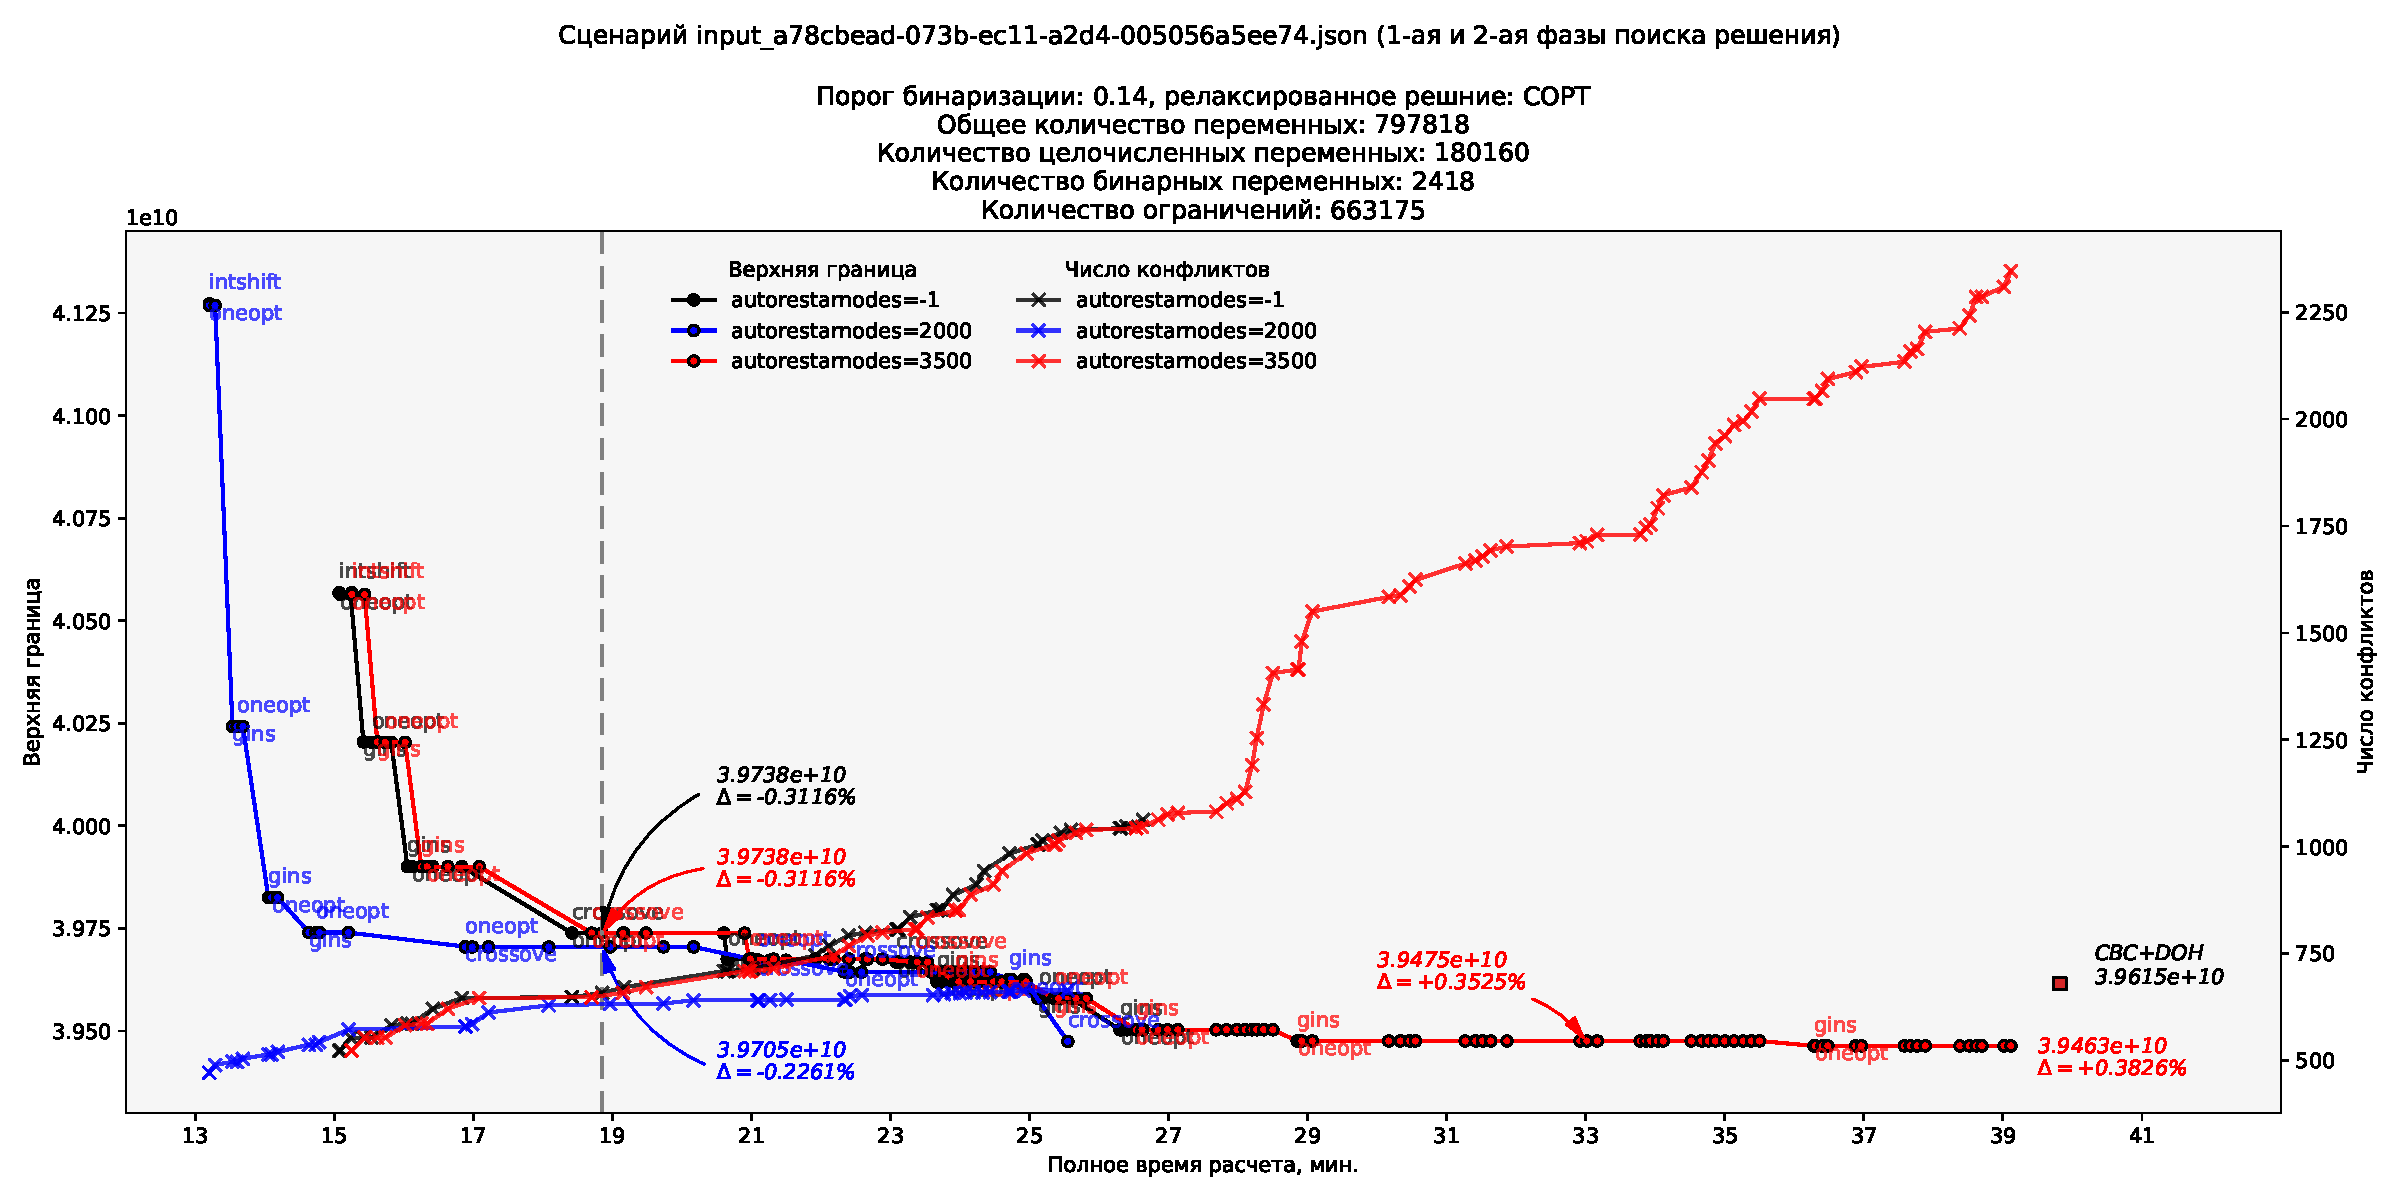
\includegraphics[scale=0.63]{figures/a78cbead_autorestartnodes_1_2_phase.pdf}
		\caption{ Динамика изменения верхней границы решения и числа конфликтов во времени в зависимости \\от значения параметра \texttt{autorestartnodes}. Сценарий \texttt{input\_a78cbead}. Первая и вторая фазы поиска решения }\label{fig:a78cbead_autorestartnodes_1_2_phase}
	\end{figure}
\end{landscape}

\begin{landscape}
\begin{figure}[!h]
	\centering
	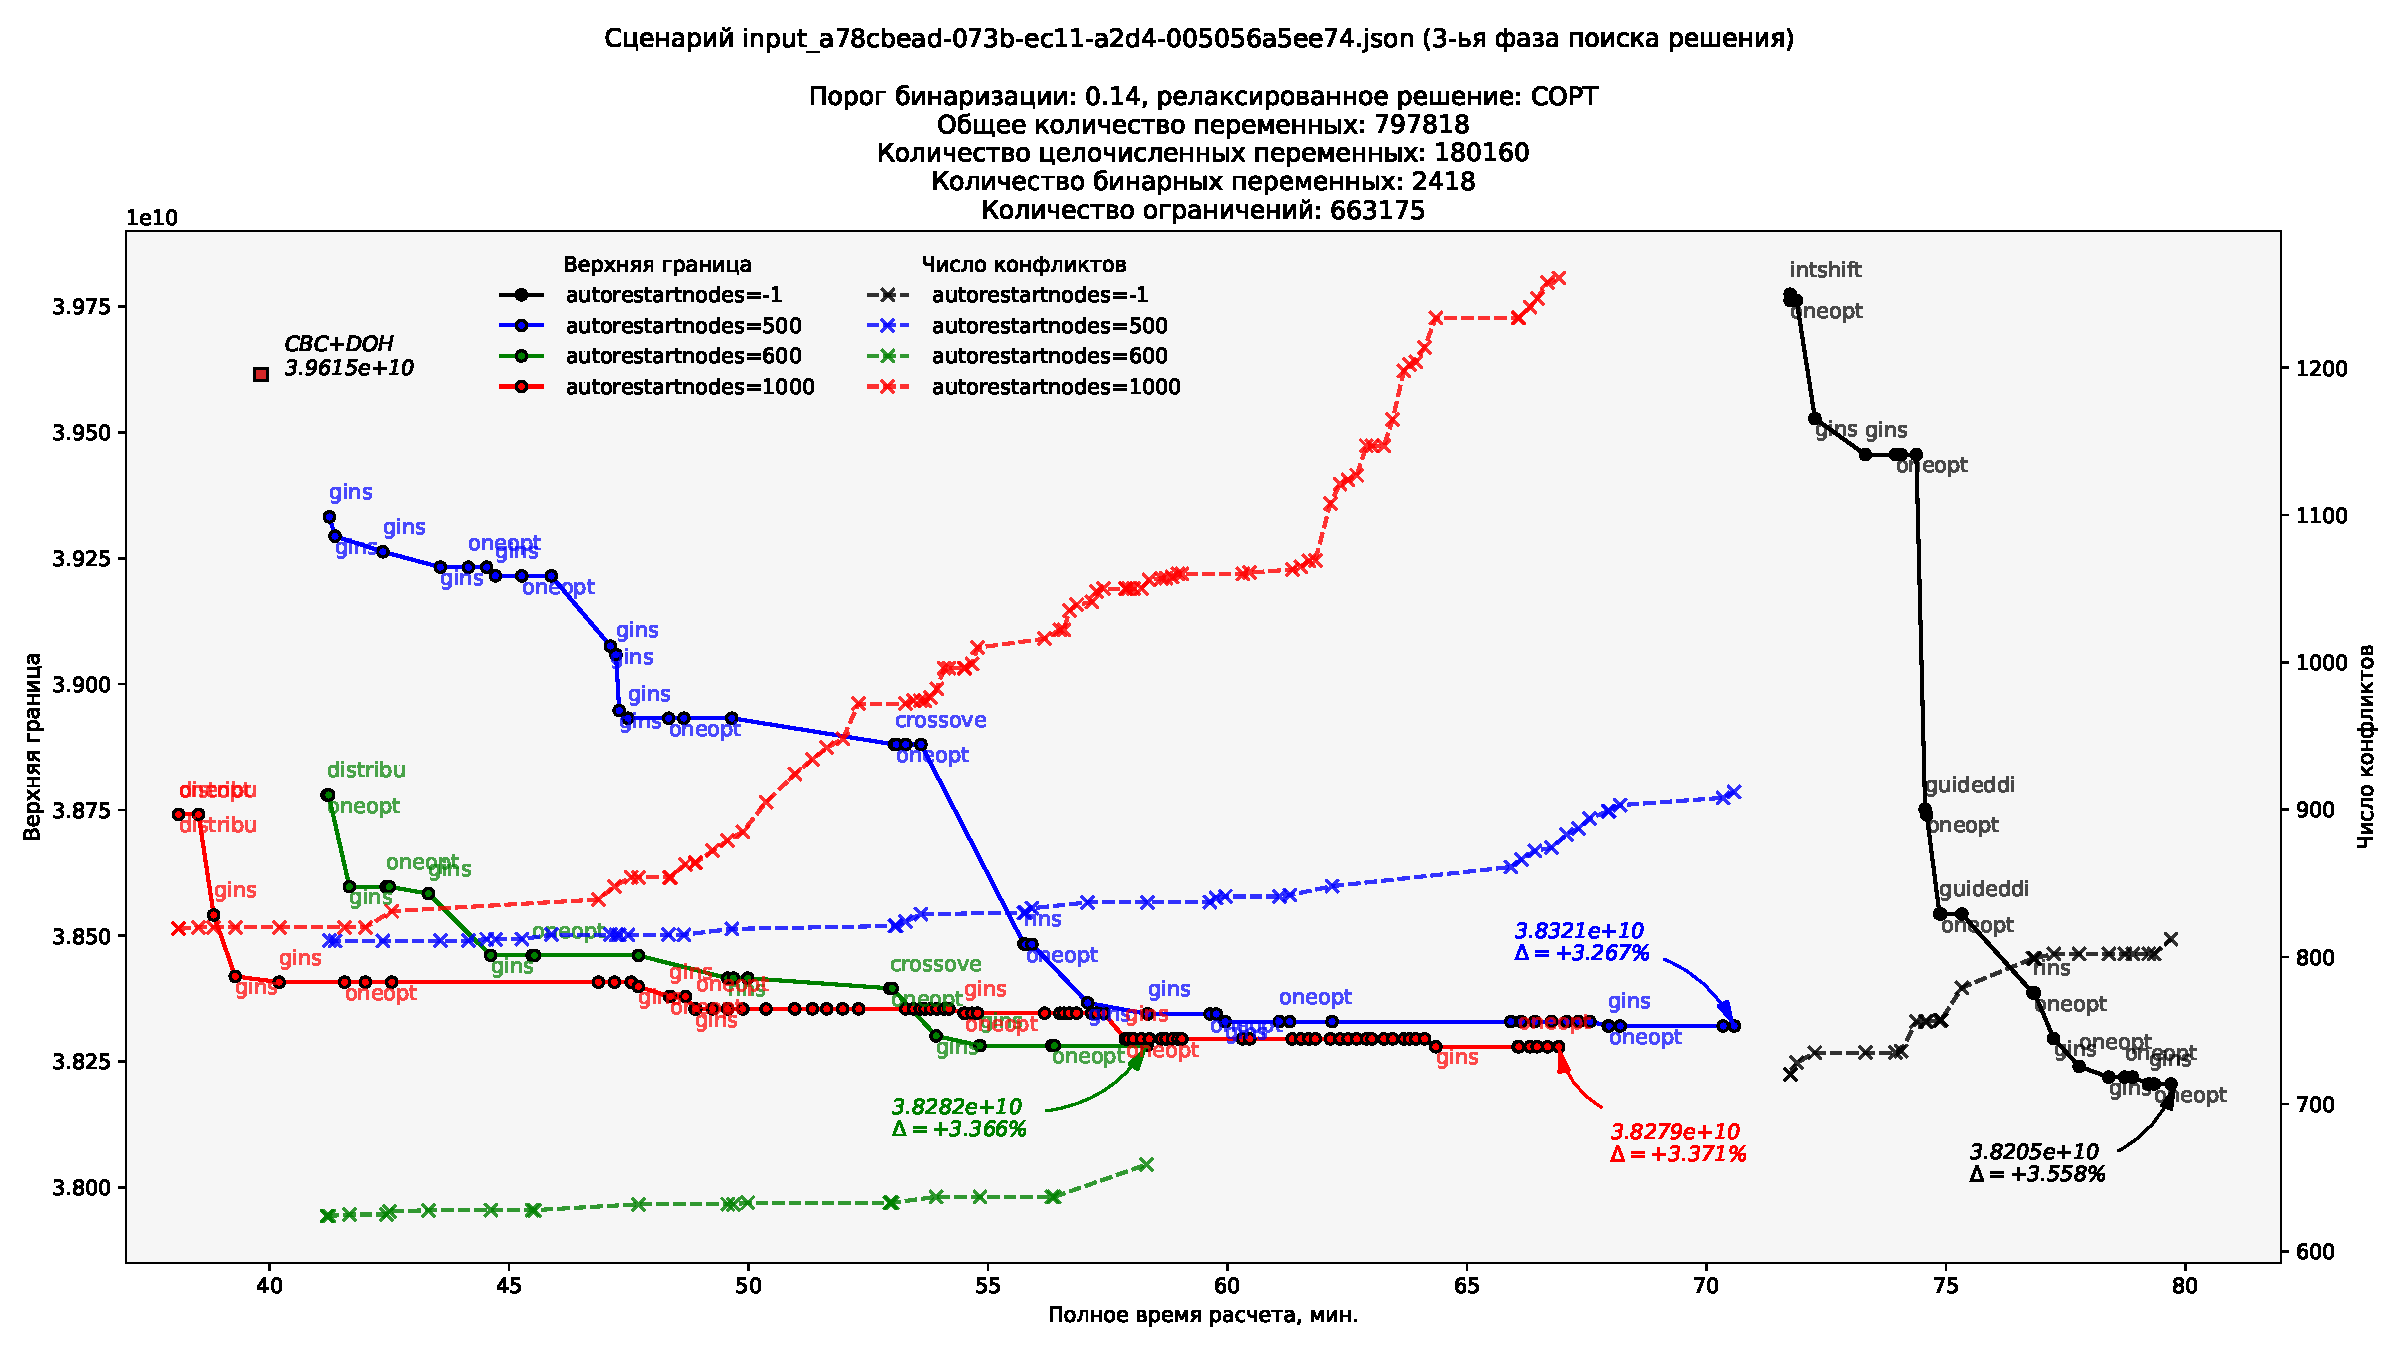
\includegraphics[scale=0.63]{figures/a78cbead_autorestartnodes_3_phase.pdf}
	\caption{ Динамика изменения верхней границы решения и числа конфликтов во времени в зависимости \\от значения параметра \texttt{autorestartnodes}. Сценарий \texttt{a78cbead}. Третья фаза поиска решения }\label{fig:a78cbead_autorestartnodes_3_phase}
\end{figure}
\end{landscape}

\begin{landscape}
\begin{figure}[!h]
	\centering
	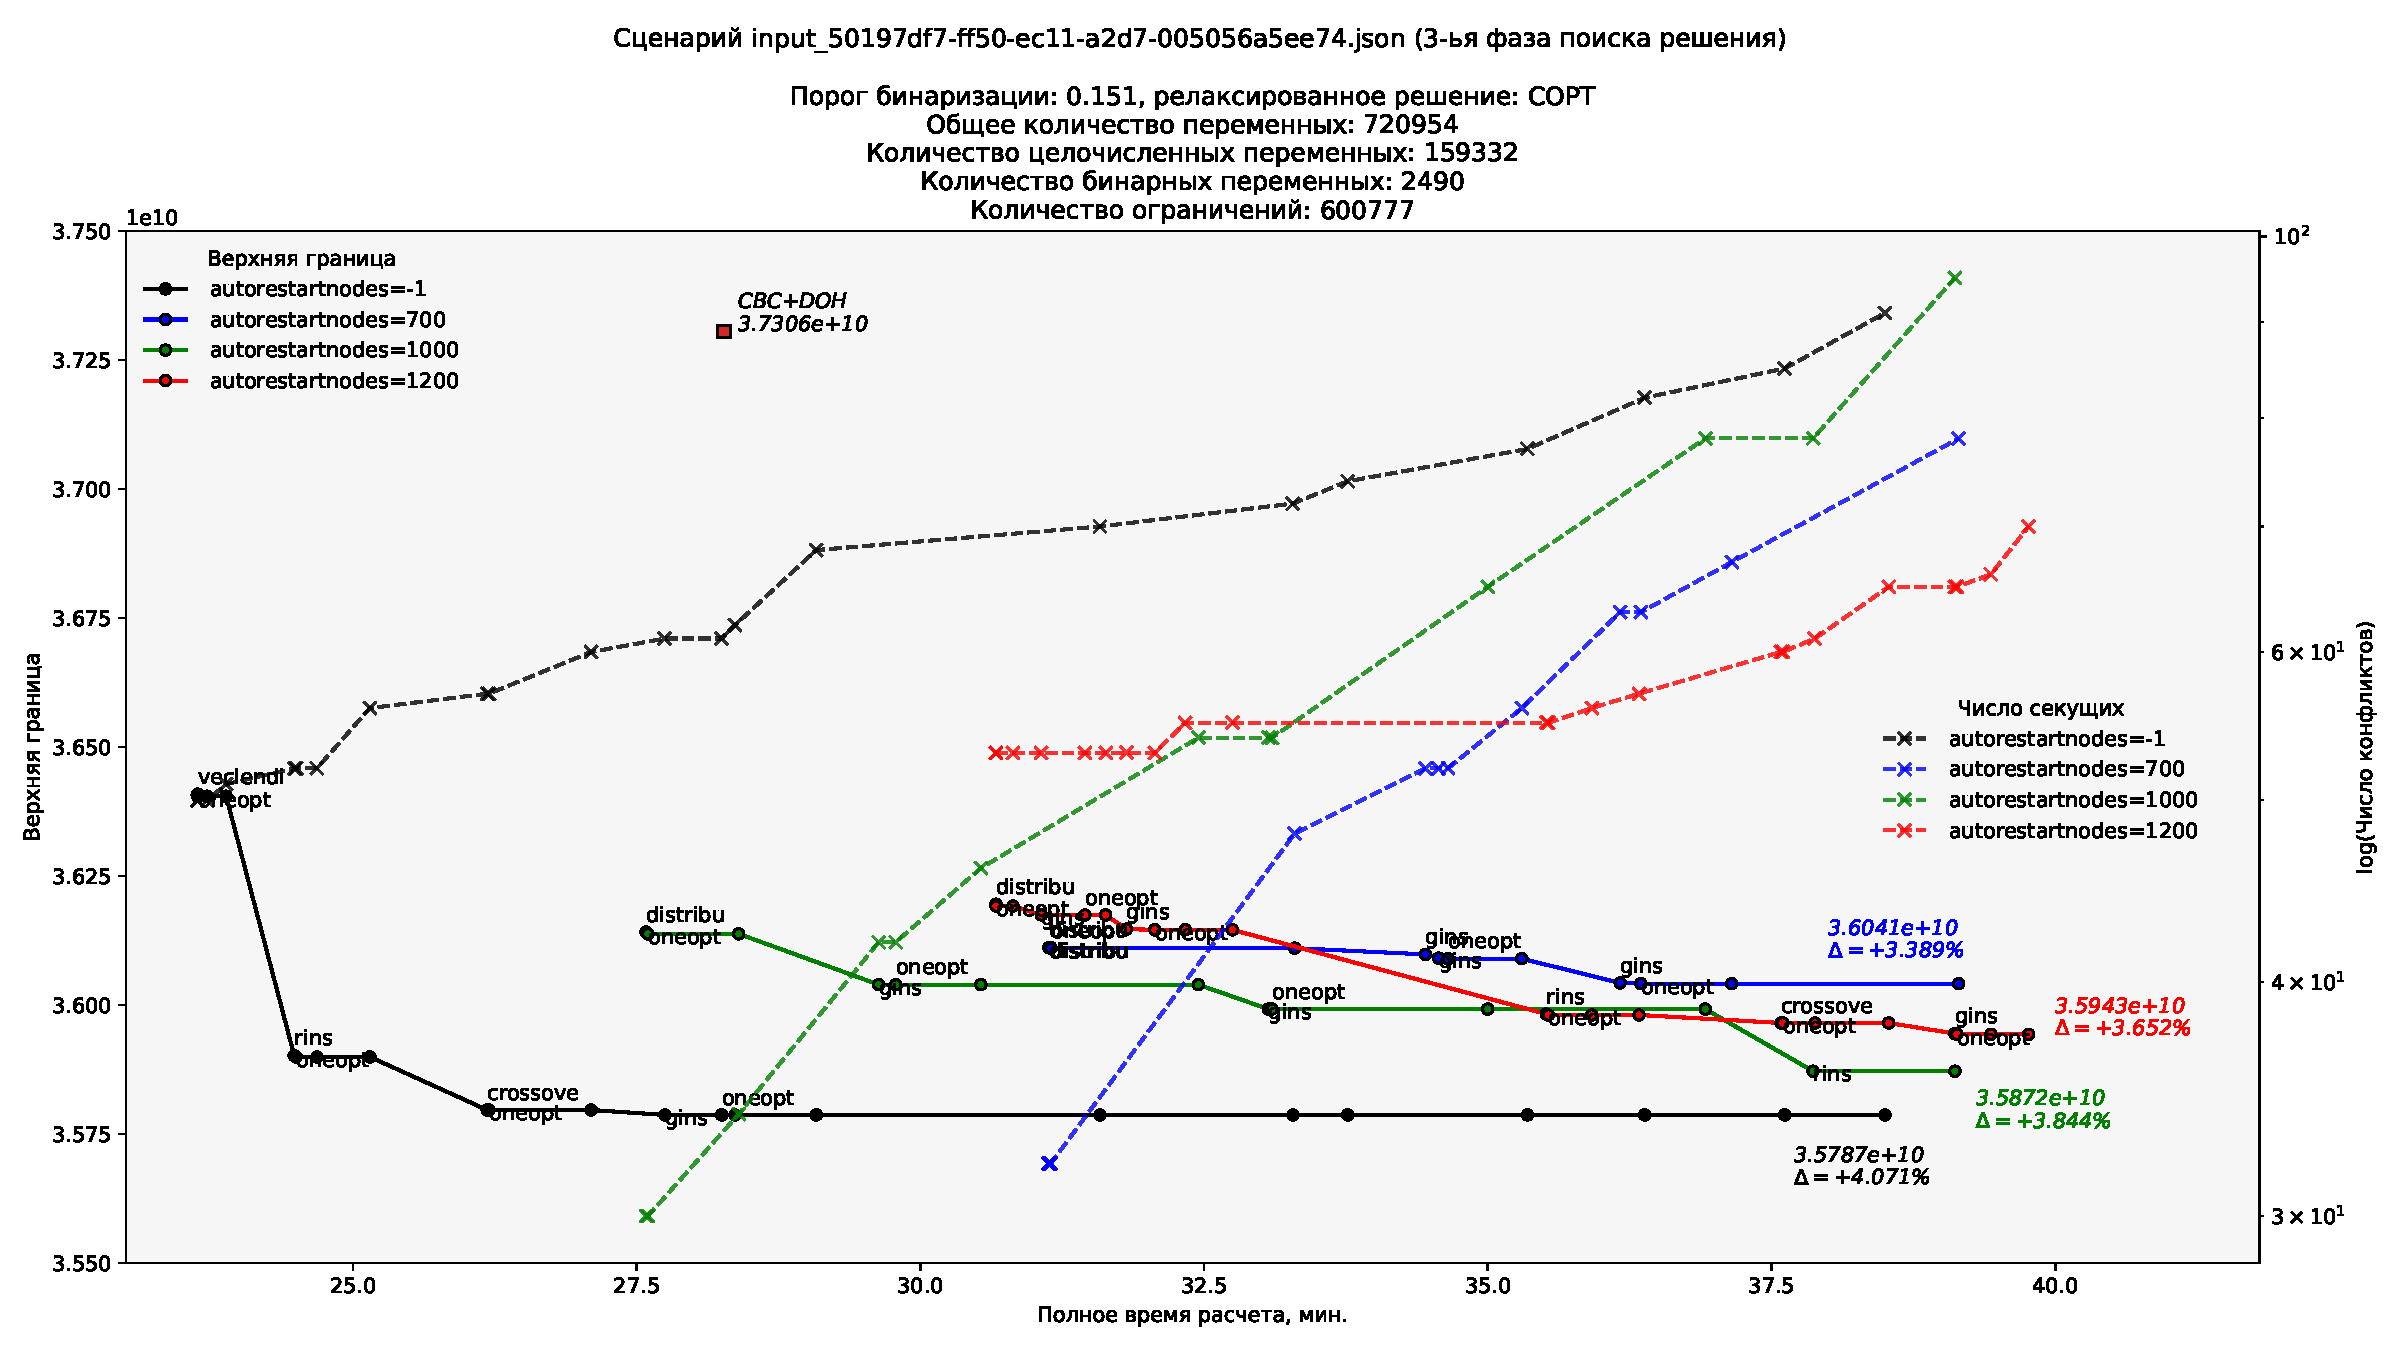
\includegraphics[scale=0.63]{figures/50197df7_autorestartnodes.pdf}
	\caption{ Динамика изменения верхней границы решения и числа конфликтов во времени в зависимости \\от значения параметра \texttt{autorestartnodes}. Сценарий \texttt{50197df7}. Третья фаза поиска решения}\label{fig:50197df7_autorestartnodes}
\end{figure}
\end{landscape}

\begin{landscape}
\begin{figure}[!h]
	\centering
	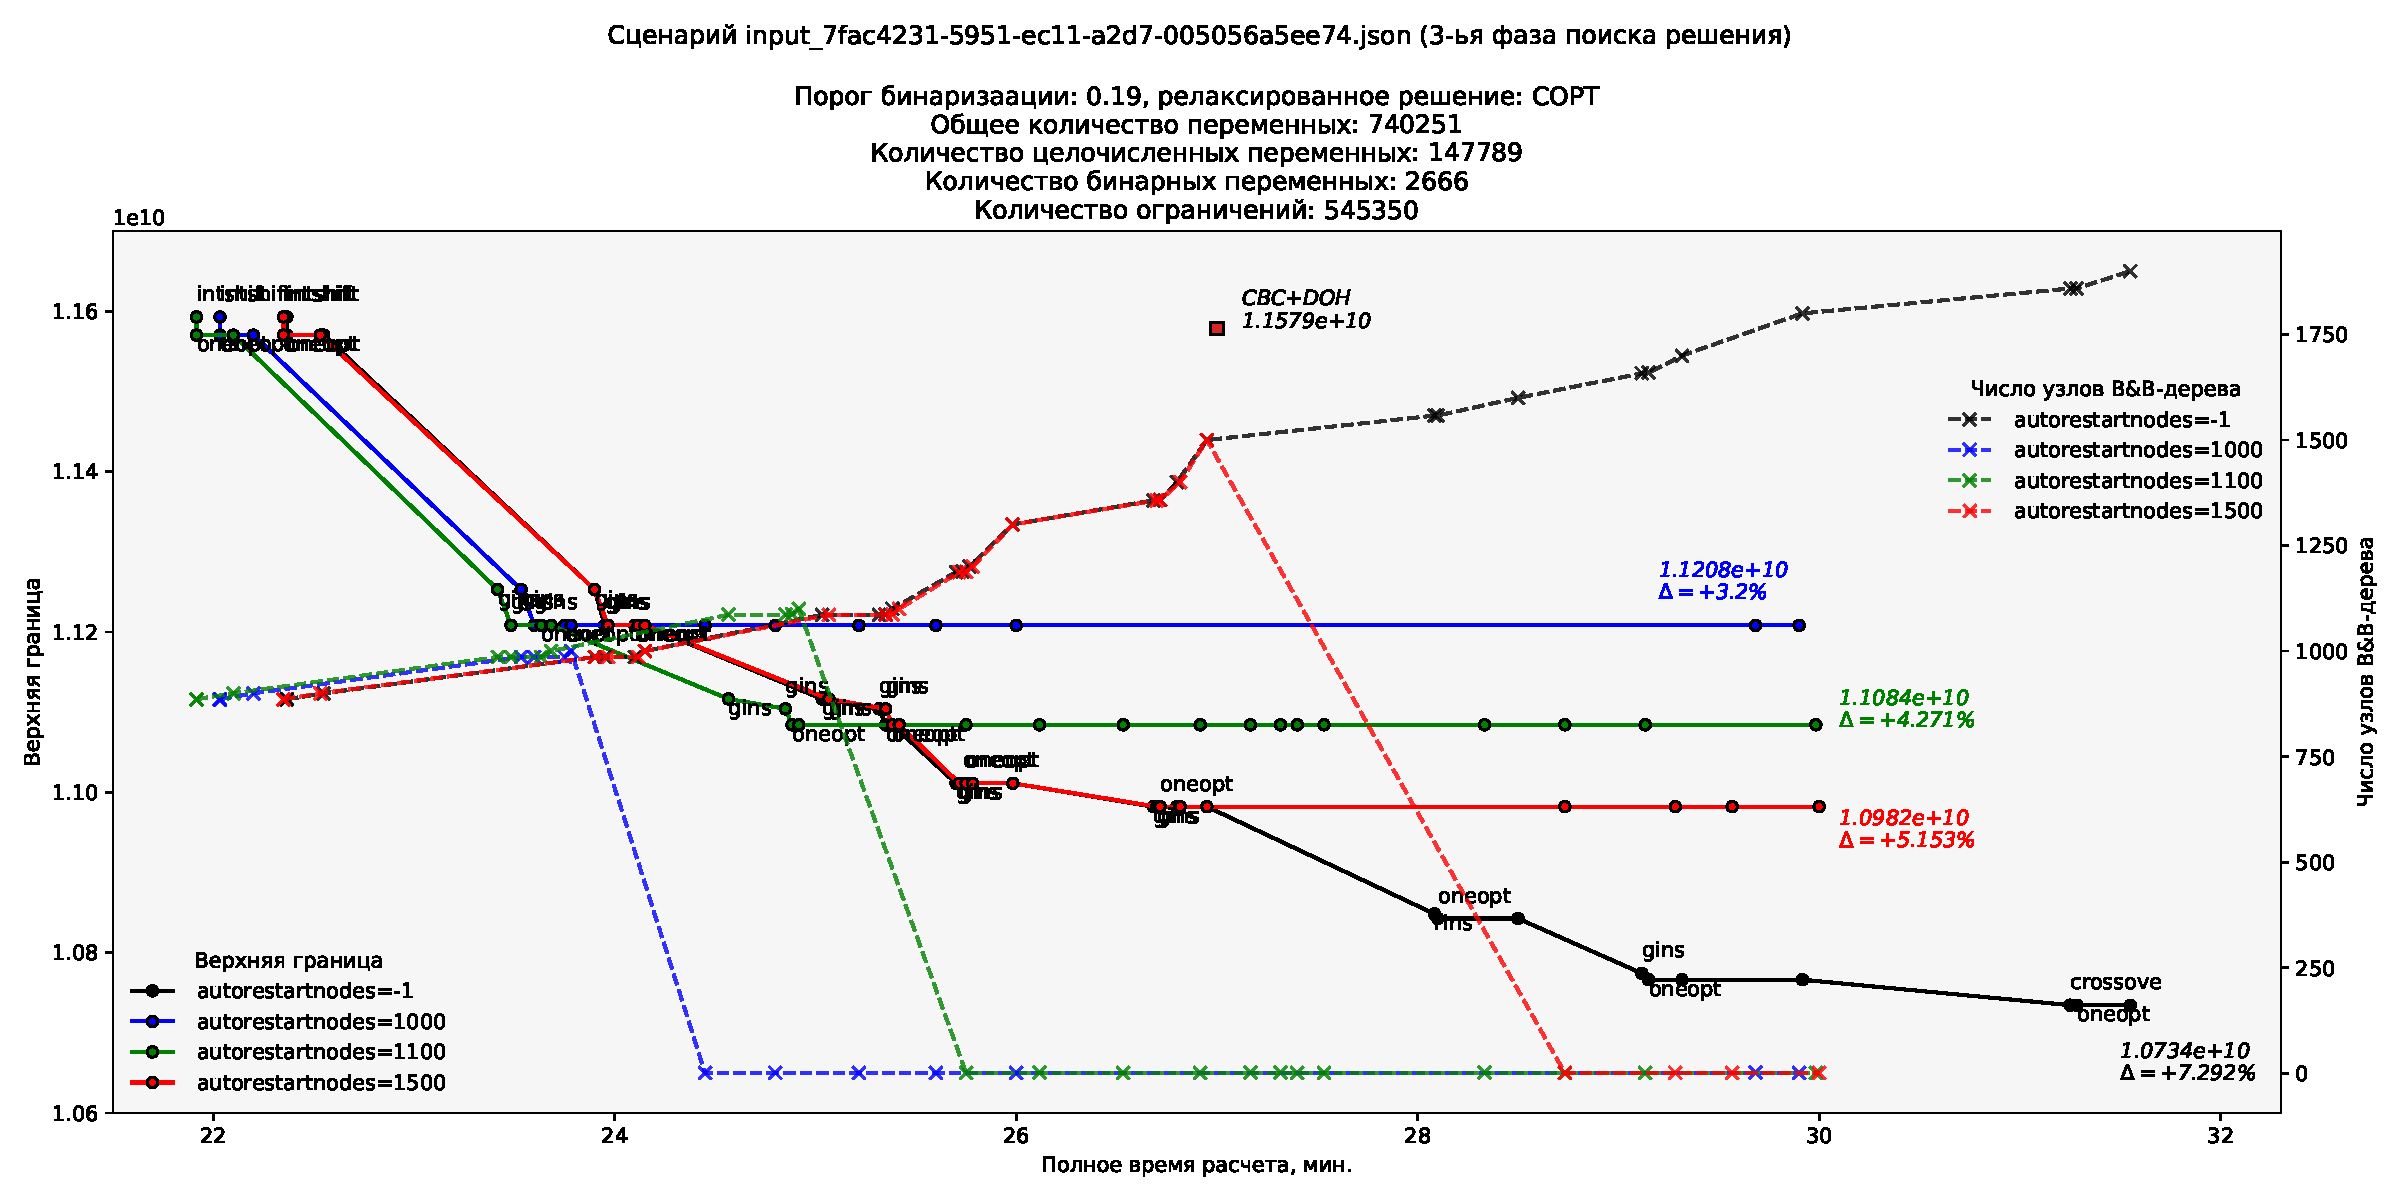
\includegraphics[scale=0.63]{figures/7fac4231_autorestartnodes.pdf}
	\caption{ Динамика изменения верхней границы решения и числа конфликтов во времени в зависимости \\от значения параметра \texttt{autorestartnodes}. Сценарий \texttt{7fac4231}. Третья фаза поиска решения}\label{fig:7fac4231_autorestartnodes}
\end{figure}
\end{landscape}


\section{Описание вычислительных экспериментов на сценариях группы MBO}

\section{Описание вычислительных экспериментов \\на сценариях MIPLIB~2017}

\subsection{Сценарии со статусом <<open>>}

\subsubsection{Сценарий \texttt{DLR2}}

\url{https://miplib.zib.de/WebData/instances/dlr2.mps.gz}

\subsubsection{Сценарий \texttt{CVRPA-N64K9VRPI}}

\url{https://miplib.zib.de/WebData/instances/cvrpa-n64k9vrpi.mps.gz}

\subsection{Сценарии со статусом <<hard>>}

\subsubsection{Сценарий \texttt{CRYPTANALYSISKB128N5OBJ14}}

\url{https://miplib.zib.de/WebData/instances/cryptanalysiskb128n5obj14.mps.gz}

\subsection{Сценарии со статусом <<easy>>}

\subsubsection{Сценарий \texttt{NEOS-4332801-seret}}

\url{https://miplib.zib.de/WebData/instances/neos-4332801-seret.mps.gz}


\newpage
\listoffigures\addcontentsline{toc}{section}{Список иллюстраций}

\listoftables\addcontentsline{toc}{section}{Список таблиц}

% Источники в "Газовой промышленности" нумеруются по мере упоминания 
\begin{thebibliography}{99}\addcontentsline{toc}{section}{Список литературы}
	\bibitem{ivanov:rl-2022}{\emph{Иванов} Конспект по обучению с подкреплением, 2022}
\end{thebibliography}

\end{document}
